% ***************************************************************************************************
%
%	Szablon pracy magisterskiej dla Politechniki Wrocławskiej w wersji dwustronnej.
%	Autor:	Tomasz Strzałka
%
% ***************************************************************************************************

% Styl dwustronny z domyślną wielkością czcionki 10pt oraz oddzieloną stroną tytułową (titlepage).
% Domyślnie rodziały rozpoczynają się na stronie prawej (openright).
\documentclass{book}

% ***************************************************************************************************
% Ustawienia języka
% ***************************************************************************************************

% Podstawowe ustawienia języka, według którego formatowany będzie dokument
\usepackage[polish]{babel}
	
% Pakiet babel dla polskiego języka powoduje konflikt z pakietem amssymb.
% Polecenie '\lll' definiują oba pakiety - porządana jest druga definicja.
\let\lll\undefined

% W przypadku wielojęzykowości ustawia główny język dokumentu
\selectlanguage{polish}

% Kodowanie dokumentu
\usepackage[utf8]{inputenc}

% Dowolny rozmiar czcionek, kodowanie znaków
\usepackage{lmodern}

% Polskie wcięcia akapitów
\usepackage{indentfirst}

% Polskie łamanie wyrazów
\usepackage[plmath]{polski}

% Przecinek w wyrażeniach matematycznych zamiast kropki
\usepackage{icomma}

% Polskie formatowanie typograficzne
\frenchspacing

% Zapewnia liczne usprawnienia wyświetlania i organizacji matematycznych formuł. 
\usepackage{amsmath}

% Wprowadza rozszerzony zestaw symboli m.in. \leadsto
\usepackage{amssymb}

% Dodatkowa, ,,kręcona'' czcionka matematyczna
\usepackage{mathrsfs}

% Dodatkowe wsparcie dla środowiska mathbb, które nie wspiera domyślnie cyfr (\mathbb{})
\usepackage{bbold}

% Fixes/improves amsmath
\usepackage{mathtools}

% Dodanie np. znaku stopni(°)
\usepackage{gensymb}

% Dla elementów z opcją [H] (force here)
\usepackage{float}

% Kolorowanie i formatowanie składni (wstawianie kodu)
\usepackage{minted}

% ***************************************************************************************************
% Kolory  
% ***************************************************************************************************

% Umożliwia kolorowanie poszczególnych komórek tabeli
\usepackage[table]{xcolor}% http://ctan.org/pkg/

% Umożliwia łatwą zmianę koloru linii w tabeli
\usepackage{tabu}

% Umożliwia rozszerzoną kontrolę nad kolorami.
\usepackage{xcolor}

% Definicje kolorów
\definecolor{lgray}{HTML}{9F9F9F}
\definecolor{dgray}{HTML}{5F5F5F}
% lgray				-	nazwa nowo zdefiniowanego koloru
% HTML				-	model kolorów
% CCCCCC			-	wartość koloru zgodna z modelem

% ***************************************************************************************************
% Algorytmy 
% ***************************************************************************************************

% Udostępnia środowisko do konstruowania pseudokodów
\usepackage[ruled,vlined,linesnumbered,longend,algochapter]{algorithm2e}
% ruled	- poziome kreski na początku i końcu algorytmu, podpis na górze oddzielony również kreską poziomą
% vlined - pionowe kreski łączące początek polecenia z jego końcem
% linesnumbered	- numerowanie kolejnych wierszy algorytmu
% longend - długie końcówki np. ifend, forend itd.
% algochapter - numeracja z rozdziałami

% Zamiana nazwy środowiska z domyślnej "Algorithm X" na "Pseudokod X"
\newenvironment{pseudokod}[1][htb]{
	\renewcommand{\algorithmcfname}{Pseudokod}
	\begin{algorithm}[#1]%
	}{
\end{algorithm}
}

% Zmiana rozmiaru komentarzy
\newcommand\algcomment[1]{
	\footnotesize{#1}
}

% Ustawienie zadanego stylu dla komentarzy
\SetCommentSty{algcomment}

% Wyśrodkowana tylda
\usepackage{textcomp}%
\newcommand{\textapprox}{\raisebox{0.5ex}{\texttildelow}}

% Listowanie kodów źródłowych
\usepackage{listings} 
\renewcommand{\lstlistingname}{Kod źródłowy} % Polska nazwa listingu


% Definicje pecjalnych znaków, które nie są obsługiwane w środowisku listing
\lstset{literate=
	{ż}{{\.{z}}}1	{ź}{{\'{z}}}1
	{ć}{{\'{c}}}1	{ń}{{\'{n}}}1
	{ą}{{\c a}}1	{ś}{{\'{s}}}1
	{ł}{{\l}}1		{ę}{{\c{e}}}1
	{ó}{{\'{o}}}1	{á}{{\'a}}1
	{é}{{\'e}}1		{í}{{\'i}}1
	{ó}{{\'o}}1		{ú}{{\'u}}1
	{ù}{{\`u}}1		{Á}{{\'A}}1
	{É}{{\'E}}1		{Í}{{\'I}}1
	{Ó}{{\'O}}1		{Ú}{{\'U}}1
	{à}{{\`a}}1		{è}{{\'e}}1
	{ì}{{\`i}}1		{ò}{{\`o}}1
	{ò}{{\`o}}1		{À}{{\`A}}1
	{È}{{\'E}}1		{Ì}{{\`I}}1
	{Ò}{{\`O}}1		{Ò}{{\`O}}1
	{ä}{{\"a}}1		{ë}{{\"e}}1
	{ï}{{\"i}}1		{ö}{{\"o}}1
	{ü}{{\"u}}1		{Ä}{{\"A}}1
	{Ë}{{\"E}}1		{Ï}{{\"I}}1
	{Ö}{{\"O}}1		{Ü}{{\"U}}1
	{â}{{\^a}}1		{ê}{{\^e}}1
	{î}{{\^i}}1		{ô}{{\^o}}1
	{û}{{\^u}}1		{Â}{{\^A}}1
	{Ê}{{\^E}}1		{Î}{{\^I}}1
	{Ô}{{\^O}}1		{Û}{{\^U}}1
	{œ}{{\oe}}1		{Œ}{{\OE}}1
	{æ}{{\ae}}1		{Æ}{{\AE}}1
	{ß}{{\ss}}1		{ç}{{\c c}}1
	{Ç}{{\c C}}1	{ø}{{\o}}1
	{å}{{\r a}}1	{Å}{{\r A}}1
	{€}{{\EUR}}1	{£}{{\pounds}}1
}

% Prezentacja drzewa katalogów
\usepackage[edges]{forest}

\definecolor{foldercolor}{RGB}{124,166,198}

\tikzset{pics/folder/.style={code={%
    \node[inner sep=0pt, minimum size=#1](-foldericon){};
    \node[folder style, inner sep=0pt, minimum width=0.3*#1, minimum height=0.6*#1, above right, xshift=0.05*#1] at (-foldericon.west){};
    \node[folder style, inner sep=0pt, minimum size=#1] at (-foldericon.center){};}
    },
    pics/folder/.default={20pt},
    folder style/.style={draw=foldercolor!80!black,top color=foldercolor!40,bottom color=foldercolor}
}

\forestset{is file/.style={edge path'/.expanded={%
        ([xshift=\forestregister{folder indent}]!u.parent anchor) |- (.child anchor)},
        inner sep=1pt},
    this folder size/.style={edge path'/.expanded={%
        ([xshift=\forestregister{folder indent}]!u.parent anchor) |- (.child anchor) pic[solid]{folder=#1}}, inner xsep=0.6*#1},
    folder tree indent/.style={before computing xy={l=#1}},
    folder icons/.style={folder, this folder size=#1, folder tree indent=3*#1},
    folder icons/.default={12pt},
}



% ***************************************************************************************************
% Marginesy 
% ***************************************************************************************************

% Ustawienia rozmiarów stron i ich marginesów
\usepackage[headheight=18pt, top=25mm, bottom=25mm, left=25mm, right=25mm]{geometry}
% headheight		-	wysokość tytułów
% top				-	margines górny
% bottom			-	margines dolny
% left				-	margines lewy
% right				-	margines prawy

% Usunięcie górnego marginesu dla środowisk
\makeatletter
\setlength\@fptop{0\p@}	
\makeatother

% ***************************************************************************************************
% Styl 
% ***************************************************************************************************

% Definiuje środowisko 'titlingpage', które zapewnia pełną kontrolę nad układem strony tytułowej.
\usepackage{titling}


% Umożliwia modyfikowanie stylu spisu treści
\usepackage{tocloft}	

\tocloftpagestyle{tableOfContentStyle}

% Definiowanie własnych stylów nagłówków i/lub stopek
\usepackage{fancyhdr}

% Domyślny styl dla pracy 
\fancypagestyle{custom}{
	\fancyhf{}									% wyczyść stopki i nagłówki
	\fancyhead[RO]{								% Prawy, nieparzysty nagłówek
		\hrulefill \hspace{16pt} \large Rozdział \thechapter
		\put(-472.1, 12.1){%
			\makebox(0,0)[l]{%
				
\includegraphics[width=0.05\textwidth]{obrazki/pwr-logo.png}
			}
		}
		\put(-443,5.5){%
			\makebox(0,0)[l]{%
				\small Politechnika Wrocławska
			}
		}
	}
	\fancyhead[LE]{								% Lewy, parzysty nagłówek
		\large Rozdział \thechapter \hspace{16pt} \hrulefill 
		\put(-22, 12.1){%
			\makebox(0,0)[l]{%
				
\includegraphics[width=0.05\textwidth]{obrazki/wppt-logo.png}
			}
		}
		\put(-210,5.5){%
			\makebox(0,0)[l]{%
				\small Wydział Podstawowych Problemów Techniki
			}
		}
	}
	\fancyfoot[LE,RO]{							% Stopki
		\thepage
	}
	\renewcommand{\headrulewidth}{0pt}			% Grubość linii w nagłówku
	\renewcommand{\footrulewidth}{0.2pt}		% Grubość linii w stopce
}


% Domyślny styl dla bibliografii
\fancypagestyle{bibliographyStyle}{
	\fancyhf{}									% wyczyść stopki i nagłówki
	\fancyhead[RO]{								% Prawy, nieparzysty nagłówek
		\hrulefill \hspace{16pt} \large Dodatek \thechapter
		\put(-472.1, 12.1){%
			\makebox(0,0)[l]{%
				
\includegraphics[width=0.05\textwidth]{obrazki/pwr-logo.png}
			}
		}
		\put(-443,5.5){%
			\makebox(0,0)[l]{%
				\small Politechnika Wrocławska
			}
		}
	}
	\fancyhead[LE]{								% Lewy, parzysty nagłówek
		\large Bibliografia \hspace{16pt} \hrulefill 
		\put(-22, 12.1){%
			\makebox(0,0)[l]{%
				
\includegraphics[width=0.05\textwidth]{obrazki/wppt-logo.png}
			}
		}
		\put(-210,5.5){%
			\makebox(0,0)[l]{%
				\small Wydział Podstawowych Problemów Techniki
			}
		}
	}
	\fancyfoot[LE,RO]{							% Stopki
		\thepage
	}
	\renewcommand{\headrulewidth}{0pt}			% Grubość linii w nagłówku
	\renewcommand{\footrulewidth}{0.2pt}		% Grubość linii w stopce
}

% Domyślny styl dla dodatków
\fancypagestyle{appendixStyle}{
	\fancyhf{}									% wyczyść stopki i nagłówki
	\fancyhead[RO]{								% Prawy, nieparzysty nagłówek
		\hrulefill \hspace{16pt} \large Dodatek \thechapter
		\put(-472.1, 12.1){%
			\makebox(0,0)[l]{%
				
\includegraphics[width=0.05\textwidth]{obrazki/pwr-logo.png}
			}
		}
		\put(-443,5.5){%
			\makebox(0,0)[l]{%
				\small Politechnika Wrocławska
			}
		}
	}
	\fancyhead[LE]{								% Lewy, parzysty nagłówek
		\large Dodatek \thechapter \hspace{16pt} \hrulefill 
		\put(-22, 12.1){%
			\makebox(0,0)[l]{%
				
\includegraphics[width=0.05\textwidth]{obrazki/wppt-logo.png}
			}
		}
		\put(-210,5.5){%
			\makebox(0,0)[l]{%
				\small Wydział Podstawowych Problemów Techniki
			}
		}
	}
	\fancyfoot[LE,RO]{							% Stopki
		\thepage
	}
	\renewcommand{\headrulewidth}{0pt}			% Grubość linii w nagłówku
	\renewcommand{\footrulewidth}{0.2pt}		% Grubość linii w stopce
}

% Osobny styl dla stron zaczynających rozdział/spis treści itd. (domyślnie formatowane jako "plain")
\fancypagestyle{chapterBeginStyle}{
	\fancyhf{}%
	\fancyfoot[LE,RO]{
		\thepage
	}
	\renewcommand{\headrulewidth}{0pt}
	\renewcommand{\footrulewidth}{0.2pt}
}

% Styl dla pozostałych stron spisu treści
\fancypagestyle{tableOfContentStyle}{
	\fancyhf{}%
	\fancyfoot[LE,RO]{
		\thepage
	}
	\renewcommand{\headrulewidth}{0pt}
	\renewcommand{\footrulewidth}{0.2pt}
}

% Formatowanie tytułów rozdziałów i/lub sekcji
\usepackage{titlesec}

% Formatowanie tytułów rozdziałów
\titleformat{\chapter}[hang]					% kształt
{
	\vspace{-10ex}
	\Huge
	\bfseries
}												% formatowanie tekstu modyfikowanego elementu
{}												% etykieta występująca przed tekstem modyfikowanego elementu, niewidoczna w spisie treści
{
	10pt
}												% odstęp formatowanego tytułu od lewego marginesu/etykiety
{
	\Huge
	\bfseries
}												% formatowanie elementów przed modyfikowanym tytułem
[
\vspace{2ex}
%\rule{\textwidth}{0.4pt}
%\vspace{-4ex}
]												% dodatkowe formatowanie stosowane poniżej modyfikowanego tytułu


% Formatowanie tytułów sekcji
\titleformat{\section}[hang]					% kształt
{
	\vspace{2ex}
%	\titlerule\vspace{1ex}
	\Large\bfseries
}												% formatowanie tekstu modyfikowanego elementu
{
	\thesection									% etykieta występująca przed tekstem modyfikowanego elementu, niewidoczna w spisie treści
}
{
	0pt
}												% odstęp formatowanego tytułu od lewego marginesu/etykiety
{
	\Large
	\bfseries
}												% formatowanie elementów przed modyfikowanym tytułem

% komenda do wpisywania źródła pod obrazkiem
\newcommand*{\captionsource}[2]{%
  \caption[{#1}]{%
    #1%
    \\\hspace{\linewidth}%
    Źródło: #2%
  }%
}

% modyfikowanie wielkości ułamka
\newcommand{\myfrac}[3][0pt]{\genfrac{}{}{}{}{\raisebox{#1}{$#2$}}{\raisebox{-#1}{$#3$}}}

% ***************************************************************************************************
% Linki
% ***************************************************************************************************

% Umożliwia wstawianie hiperłączy do dokumentu
\usepackage{hyperref}							% Aktywuje linki

\hypersetup{
	colorlinks	=	true,					% Koloruje tekst zamiast tworzyć ramki.
	linkcolor		=	blue,					% Kolory: referencji,
        citecolor		=	blue,					% cytowań,
	urlcolor		=	blue					% hiperlinków.
}

% Do stworzenia hiperłączy zostanie użyta ta sama (same) czcionka co dla reszty dokumentu
\urlstyle{same}




% ***************************************************************************************************
% Linki

% ***************************************************************************************************

% Umożliwia zdefiniowanie własnego stylu wyliczeniowego
\usepackage{enumitem}

% Nowa lista numerowana z trzema poziomami
\newlist{myitemize}{itemize}{3}

% Definicja wyglądu znacznika pierwszego poziomu
\setlist[myitemize,1]{
	label		=	\textbullet,
	leftmargin	=	4mm}

% Definicja wyglądu znacznika drugiego poziomu
\setlist[myitemize,2]{
	label		=	$\diamond$,
	leftmargin	=	8mm}

% Definicja wyglądu znacznika trzeciego poziomu
\setlist[myitemize,3]{
	label		=	$\diamond$,
	leftmargin	=	12mm
}

% ***************************************************************************************************
% Inne pakiety
% ***************************************************************************************************

% Dołączanie rysunków
\usepackage{graphicx}

% Dołączanie SVG
\usepackage{svg}
\svgsetup{inkscapelatex=false} % nie konwertuj tekstu używając LaTeXa

% Figury i przypisy
\usepackage{caption}
\usepackage{subcaption}

% Umożliwia tworzenie przypisów wewnątrz środowisk
\usepackage{footnote}

% Umożliwia tworzenie struktur katalogów
\usepackage{dirtree}

% Rozciąganie komórek tabeli na wiele wierszy
\usepackage{multirow}


% Precyzyjne obliczenia szerokości/wysokości dowolnego fragmentu wygenerowanego przez LaTeX
\usepackage{calc}

% ***************************************************************************************************
% Matematyczne skróty
% ***************************************************************************************************

% Skrócony symbol liczb rzeczywistych
\newcommand{\RR}{\mathbb{R}}

% Skrócony symbol liczb naturalnych
\newcommand{\NN}{\mathbb{N}}
 
% Skrócony symbol liczb wymiernych
\newcommand{\QQ}{\mathbb{Q}}

% Skrócony symbol liczb całkowitych
\newcommand{\ZZ}{\mathbb{Z}}

% Skrócony symbol logicznej implikacji
\newcommand{\IMP}{\rightarrow}

% Skrócony symbol  logicznej równoważności
\newcommand{\IFF}{\leftrightarrow}

% ***************************************************************************************************
% Środowiska
% ***************************************************************************************************

% Środowisko do twierdzeń
\newtheorem{theorem}{Twierdzenie}[chapter]

% Środowisko do lematów
\newtheorem{lemma}{Lemat}[chapter]

% Środowisko do przykładów
\newtheorem{example}{Przykład}[chapter]

% Środowisko do wniosków
\newtheorem{corollary}{Wniosek}[chapter]

% Środowisko do definicji
\newtheorem{definition}{Definicja}[chapter]

% Środowisko do pytań
\newtheorem{question}{Pytanie}[chapter]

% Środowisko do dowodów
\newenvironment{proof}{
	\par\noindent \textbf{Dowód.}
}{
\begin{flushright}
	\vspace*{-6mm}\mbox{$\blacklozenge$}
\end{flushright}
}

% Środowisko do uwag
\newenvironment{remark}{
	\bigskip \par\noindent \small \textbf{Uwaga.}
}{
\begin{small}
	\vspace*{4mm}
\end{small}
}

% ***************************************************************************************************
% Słownik
% ***************************************************************************************************

% Prawidłowe dzielenie wyrazów
\hyphenation{wszy-stkich ko-lu-mnę każ-da od-leg-łość
	dzie-dzi-ny dzie-dzi-na rów-nych rów-ny
	pole-ga zmie-nna pa-ra-met-rów wzo-rem po-cho-dzi
	o-trzy-ma wte-dy wa-run-ko-wych lo-gicz-nie
	skreś-la-na skreś-la-ną cał-ko-wi-tych wzo-rów po-rzą-dek po-rząd-kiem
	przy-kład pod-zbio-rów po-mię-dzy re-pre-zen-to-wa-ne
	rów-no-waż-ne bi-blio-te-kach wy-pro-wa-dza ma-te-ria-łów
	prze-ka-za-nym skoń-czo-nym moż-esz na-tu-ral-na cią-gu tab-li-cy
	prze-ka-za-nej od-po-wied-nio}

% ***************************************************************************************************
% Dokument
% ***************************************************************************************************

\frontmatter

\begin{document}

	\begin{titlingpage}
		\vspace*{\fill}
		\begin{center}
			\begin{picture}(300,510)
				\put(11,520){\makebox(0,0)[l]{\large \textsc{Wydział Podstawowych Problemów Techniki}}}
				\put(11,500){\makebox(0,0)[l]{\large \textsc{Politechnika Wrocławska}}}
% Tytuł pracy
				\put(80,400){\Huge \textsc{System wspomagający}}
				\put(80,360){\Huge \textsc{grę w darta}}
				\put(80,320){\Huge \textsc{z wykorzystaniem}}
				\put(80,280){\Huge \textsc{analizy obrazu}}
				\put(80,240){\Huge \textsc{w czasie rzeczywistym}}
% Autor pracy
				\put(90,200){\makebox(0,0)[l]{\large \textsc{Piotr Andrzejewski}}}
				\put(90,180){\makebox(0,0)[l]{\large \textsc{Nr indeksu: 244931}}}

				\put(200,100){\makebox(0,0)[l]{\large Praca inżynierska napisana}}
				\put(200,80){\makebox(0,0)[l]{\large pod kierunkiem}}
% dane promotora
				\put(200,60){\makebox(0,0)[l]{\large dr. inż. Marcina Zawady}}
				
				\put(115,-70){
\includegraphics[width=0.15\textwidth]{obrazki/pwr.png}}
				\put(106,-80){\makebox(0,0)[bl]{\large \textsc{Wrocław 2020}}}
			\end{picture}
		\end{center}	
		\vspace*{\fill}
	\end{titlingpage}
	
        \cleardoublepage
		
	\pagenumbering{Roman}
	\pagestyle{tableOfContentStyle}
	\tableofcontents
	\cleardoublepage
		
	% ***************************************************************************************************
	% Wstęp
	% ***************************************************************************************************
	
	\pagestyle{custom}
	\mainmatter
	
	% ***************************************************************************************************
	% Rozdziały
	% ***************************************************************************************************

	\chapter{Wstęp}
\thispagestyle{chapterBeginStyle}

Niniejsza praca prezentuje cały proces prowadzący do automatycznego naliczania punktów w grze w darta za pomocą kamer. Obejmuje to zarówno analizę problemu, obliczenia stojące za użytą metodą, jak i projekt oraz implementację systemu. 

Celem pracy jest zaprojektowanie oraz wykonanie systemu o następujących wymaganiach:
\vspace{2mm}

\noindent a) funkcjonalnych:
\begin{itemize}
  \item wykrywanie momentu wbicia rzutki
  \item obliczanie pozycji wbitej rzutki
  \item analiza kilku rzutów bez konieczności wyciągania lotek z tarczy
  \item wyświetlanie informacji dotyczących rzutu w aplikacji mobilnej
  \item zaznaczanie pozycji rzutki na diagramie tarczy
  
\end{itemize}

\noindent b) niefunkcjonalnych:
\begin{itemize}
  \item działanie w czasie rzeczywistym, pozwalające na płynną grę
  \item niski koszt
  \item duże możliwości konfiguracji
\end{itemize}

Należy podkreślić, że system ma duży potencjał i możliwości zastosowania, ponieważ jest niewiele podobnych rozwiązań na rynku. Pojedyncze, istniejące implementacje dla profesjonalistów (np. system \textit{Scolia}\footnote{Adres: \url{https://scoliadarts.com/}}) gwarantują prawie stuprocentową skuteczność, lecz ich cena jest bardzo wysoka, a kod źródłowy i szczegóły budowy urządzenia nie są dostępne.

Praca składa się z pięciu rozdziałów. W rozdziale pierwszym poddano problem analizie, omawiając podstawy gry w darta, sposób reprezentacji rzutu oraz istniejące ograniczenia. Rozdział drugi przedstawia pomysł na rozwiązanie problemu, w pełni opisuje teoretyczny proces uzyskania pozycji rzutki na tarczy. Wytłumaczone są w nim podstawowe pojęcia oraz obliczenia prowadzące do osiągnięcia celu pracy. W rozdziale trzecim zawarte zostały opis urządzeń użytych w systemie, diagramy UML oraz algorytm przetwarzania obrazu. Rozdział czwarty traktuje o szczegółach implementacyjnych: technologiach użytych w projekcie, strukturze projektu i opisie plików źródłowych. Omówiony został tam również, na przykładzie, efekt końcowy działania programu, testy dokładności oraz problemy, które pojawiły się w trakcie implementacji. W rozdziale piątym pokazano, w jaki sposób należy zainstalować potrzebne zależności oraz uruchomić aplikację. Ostatni rozdział podsumowuje pracę, omawiając, co zostało zrealizowane i jakie są możliwe ścieżki rozwoju projektu.
	\cleardoublepage

% TODO: zdecyduj się na jednolity czas: przeszły/teraźniejszy/przyszły?
	\chapter{Analiza problemu}
\thispagestyle{chapterBeginStyle}
\label{rozdzial1}

W tym rozdziale przeanalizowano problemy zawarte w tematyce niniejszej pracy oraz przedstawiono wszystkie okoliczności, w jakich system będzie funkcjonował. Omówiono podstawy gry w darta, potrzebne do zrozumienia trudności, którym trzeba sprostać przy projektowaniu i implementacji systemu. Następnie głębiej zbadano wymagania funkcjonalne, wymienione we wstępie. Zostały wprowadzone pewne matematyczne modele, które pomogą w reprezentacji rozwiązania. Podano cel stworzenia aplikacji mobilnej i jej role. Dokładnej analizie zostały poddane ograniczenia i wymagania niefunkcjonalne systemu.

\section{Gra w darta}

Dart, znany w Polsce również pod nazwą ,,rzutki'' lub ,,lotki'', jest grą, w której zawodnicy rzucają lotkami do oddalonej od nich tarczy, w celu zdobycia punktów. 

Tarcza, zazwyczaj wykonana z sizalu, znajduje się na wysokości 173 cm, w odległości 237 cm od gracza. Ma kształt koła o średnicy 45 cm i składa się z pól, którym przyporządkowane są wartości punktowe. Dzieli się ona na 20 wycinków kołowych, punktowanych od 1 do 20 (pola standardowe). Są one jednak przecięte dwoma pierścieniami: \textit{double} (zewnętrznym) i \textit{treble} (wewnętrznym). Trafienie w zewnętrzny pierścień oznacza podwojenie liczby punktów przypisanych do danego pola standardowego, a wewnętrzny -- potrojenie. Na tarczy znajdują się także segmenty \textit{inner bull}, czyli koło znajdujące się w środku, dające 50 punktów oraz \textit{outer bull} -- pierścień okalający środkowe koło, za którego trafienie przyznaje się 25 punktów. Rzut poza wymienione pola jest liczony za zero punktów. Tarcza wraz z liczbą punktów przypisaną do każdego z pól jest pokazana na rysunku \ref{tarcza_punktacja}.

\hspace{1cm}

\begin{figure}[h!]
\begin{center}
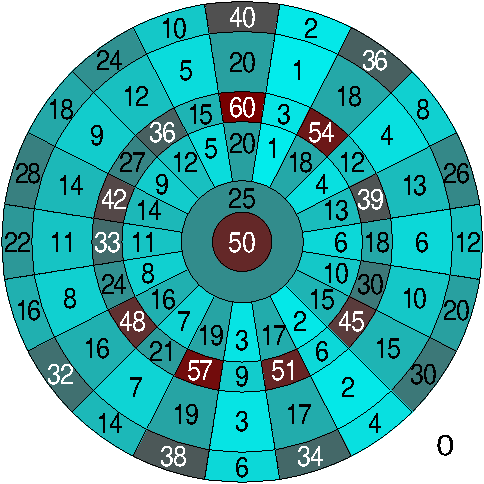
\includegraphics[width=0.4\textwidth]{obrazki/tarcza.pdf}
\end{center}
\captionsource{{\color{dgray}Tarcza do darta z przypisaniem punktów}}{Cmglee, CC BY-SA 4.0, https://commons.wikimedia.org/w/index.php?curid=49462410}
\label{tarcza_punktacja}
\end{figure} 

Najpopularniejszym wariantem darta jest \textit{501}, w którym gracze rozpoczynają rozgrywkę, mając na koncie 501 punktów. Każdy z nich wykonuje w jednej turze 3 rzuty, a suma zdobytych punktów jest odejmowana od stanu ich konta. Wygrywa ten, kto jako pierwszy osiągnie dokładnie 0 punktów. Innym znanym wariantem jest \textit{Round The Clock} -- gracze mają za zadanie trafić w każde pole na tarczy z zakresu od 1 do 20 w kolejności zgodnej z ruchem wskazówek zegara, a na końcu w pole \textit{inner bull} (tj. 20, 1, 18, \ldots, 12, 5, 50).

\section{Wykrycie rzutu i przypisanie do segmentu} \label{reprezentacja_pola}
Głównym problemem, jakim zajmuje się niniejsza praca, jest wykrycie rzutu przez system, a następnie uzyskanie segmentu, w jaki trafiła lotka. Po włączeniu systemu powinien on nieustannie analizować dane wejściowe i wysyłać sygnał, gdy rozpozna, że rzutka wbiła się w tarczę. Sygnał ten rozpocznie procesowanie danych wejściowych pod kątem obliczenia konkretnej pozycji rzutki. Najczęstszy scenariusz gry w darta wygląda tak, że każdy z graczy rzuca kolejno 3 razy, wyciąga swoje rzutki i tura przechodzi na kolejnego gracza. Z tego powodu do wygody użytkowania potrzebna jest obsługa kilku rzutów (przynajmniej trzech) bez wyciągania rzutki po każdym rzucie. Idealną sytuacją byłaby taka, gdyby bez interwencji użytkownika system był w stanie reagować na poprawne rzuty, ale ignorować wyciąganie lotek z tarczy pomiędzy turami.

Docelową daną wyjściową, którą ma dostarczać system, jest numer jednego z segmentów tarczy. W tym wypadku, zbiorem możliwych rozwiązań byłby \[W = \{0, 25, 50\} \cup A \cup B \cup C, \textrm{ gdzie } A = \{1, \ldots, 20 \}, B = \{2 \cdot a : a \in A \}, C = \{3 \cdot a : a \in A \}.\] Trzeba jednak zauważyć, że taki sposób reprezentacji powodowałby stratę pewnych informacji. Mianowicie, dla każdego $w \in (A \cap B) \cup (A \cap C) \cup (B \cap C)$  nie można by było jednoznacznie stwierdzić, jaki segment na tarczy reprezentuje. Przykładowo, pole numer 14 z podwójnego pierścienia (podwojona siódemka), byłoby tak samo przedstawiane jak standardowe pole 14. Należy zatem doprecyzować sposób reprezentacji rzutu: każdy rzut jest przedstawiany jako para $(w, t)$, gdzie $w \in W$ to liczba punktów za rzut, a $t \in \{ S, D, T \}$. $S$ oznacza pole standardowe ($\in A \cup \{0, 25, 50\}$), $D$ -- pole podwójne (\textit{double}, $\in B$), $T$ -- pole potrójne (\textit{triple}, $\in C$). Dzięki temu unika się wyżej przedstawionej niejednoznaczności: jeden segment oznacza się jako $(14, D)$, a drugi jako $(14, S)$.

Dodatkowo, przydatne może okazać się zapisanie również pośredniej reprezentacji pozycji rzutki, nie jako konkretnego pola na tarczy, ale dokładnego punktu wbicia. Nie każde rozwiązanie wymaga posiadania takich informacji, ale większość prawdopodobnie będzie je musiała wyliczyć. W takiej sytuacji punkt można przedstawiać za pomocą:
\begin{enumerate}[label=(\alph*)]
	\item współrzędnych kartezjańskich, tj. $(x, y)$, gdzie punkt $(0, 0)$ to np. lewy górny róg kwadratu opisanego na okręgu tarczy
	\item współrzędnych biegunowych, tj. $(r, \varphi)$, gdzie biegunem $O$ jest środek tarczy, a oś biegunowa $OS$ przechodzi przez punkt $S$ -- najbardziej wysunięty na prawo punkt tarczy 
\end{enumerate}
Oba podejścia są pokazane na rysunku \ref{tarcza_polozenie}.

\begin{figure}[h!]
\centering
\begin{subfigure}{.5\textwidth}
  \centering
  \includesvg[width=.8\linewidth]{obrazki/tarcza_kartezjanskie.svg}
  \caption{współrzędne kartezjańskie}
  \label{tarcza_kartezjanskie}
\end{subfigure}%
\begin{subfigure}{.5\textwidth}
  \centering
  \includesvg[width=.8\linewidth]{obrazki/tarcza_biegunowe.svg}
  \caption{współrzędne biegunowe}
  \label{tarcza_biegunowe}
\end{subfigure}
\captionsource{{\color{dgray}Rodzaje reprezentacji pozycji rzutki.}}{Opracowanie własne.}
\label{tarcza_polozenie}
\end{figure}

\section{Aplikacja mobilna}
Dodatkową częścią systemu jest aplikacja mobilna, która ma na celu atrakcyjną prezentację danych użytkownikowi, urozmaicenie rozgrywki oraz poprawę użyteczności (\textit{user experience}). W wersji podstawowej, będzie ona przede wszystkim stanowić interfejs graficzny dla systemu wbudowanego. Dzięki aplikacji mobilnej, będzie można oglądać wyniki poszczególnych rzutów oraz oglądać miejsca wbicia rzutki na wirtualnej tarczy. W rozbudowanej wersji, można do aplikacji dodać wiele innych funkcjonalności, np. wpływanie na stan gry lub wyświetlanie statystyk. 
 
\section{Ograniczenia}
Podczas tworzenia systemu należy pamiętać o ograniczeniach, które należy spełnić, by osiągnąć wszystkie wymagania, również te niefunkcjonalne. Oczywistym ograniczeniem, a jednocześnie wyznacznikiem jakości jest dokładność analizy rzutu. Może być wyrażona w różny sposób, ale ma na celu ukazanie, jak duże i/lub częste są błędy w określaniu pozycji rzutki. Bez względu na rozwiązanie, dokładność może wahać się i zależeć od wielu czynników, jednakże uśrednione dane dają natychmiastową informację o tym, na ile użyteczny jest to moduł. Głównym celem niniejszej pracy nie jest maksymalizowanie dokładności, lecz powinna być ona na poziomie pozwalającym na podstawową rozgrywkę.  

% TODO: dodać przypis do definicji czasu rzeczywistego, ew. poprawić
Innym, istotnym wskaźnikiem działania systemu jest szybkość jego działania. Jednym z celów jest możność opisania go jako \textit{system czasu rzeczywistego}. Oznacza to, że jego poprawność nie zależy jedynie od dokładności zwracanych wyników, lecz również od czasu, jaki upłynął od nadejścia danych wejściowych do otrzymania wyniku. Sytuacja z analizą rzutów odzwierciedla taką sytuację -- gracz nie chce rzucać wielu rzutek, a następnie, po czasie, zobaczyć statystyki rzutów. Aplikacja powinna działać na zasadzie akcja-reakcja: po każdym z rzutów, w krótkim czasie, powinna się pojawić informacja o wyniku. Efektem pożądanym jest sytuacja, gdy gracz nie będzie musiał czekać z następnym rzutem na zakończenie analizy poprzedniego. W przypadku, gdy oczekiwanie na wynik będzie zbyt długie, system stanie się bezużyteczny, nawet jeśli rezultaty będą bardzo dokładne. Należy zachować balans pomiędzy dokładnością a szybkością działania programu.

Rozwiązanie powinno być łatwo i szeroko konfigurowalne. Z pewnością pojawią się w nim parametry specyficzne dla np. konkretnej tarczy lub rzutek. Wszystkie tego typu części należy dobrze udokumentować oraz zapewnić prostotę modyfikacji, tak by jeden kod źródłowy mógł być z łatwością używany przez wiele osób, nawet jeśli ich lokalne parametry nie pokrywają się z tymi, które występowały u autora rozwiązania. 

Ostatnią, bardziej pragmatyczną restrykcją jest kwestia ceny całego przedsięwzięcia. Tym, co ma wyróżniać niniejsze rozwiązanie od innych jest fakt, że będzie wykonane przy użyciu łatwo dostępnych i możliwie tanich komponentów.
	\cleardoublepage

	\chapter{Teoretyczne rozwiązanie problemu}
\thispagestyle{chapterBeginStyle}

Ten rozdział ma za zadanie przedstawić teoretyczną (matematyczną) część rozwiązania głównego problemu -- uzyskania pozycji rzutki. Na początku zaprezentowany i podzielony na części został ogólny pomysł rozwiązania. Pokazane zostały również alternatywne propozycje podejścia do problemu, wraz z uzasadnieniem, dlaczego nie zostały one wybrane. Następnie omówiono podstawowe terminy i zagadnienia, których znajomość potrzebna jest do pełnego zrozumienia dalszych tematów. Główną częścią rozdziału jest prezentacja wszystkich kluczowych obliczeń i operacji, które zachodzą podczas analizy rzutu, krok po kroku. Detale dotyczące niektórych algorytmów zostaną przedstawione w późniejszych rozdziałach, w tym zaś uznaje się je za tzw. czarne skrzynki (ang. \textit{black box}), to znaczy elementy programu, które przyjmują pewne dane wejściowe i zwracają wyniki, lecz ich implementacja nie jest rozważana.

\section{Idea rozwiązania}
Pierwszą decyzją, jaką należało podjąć podczas tworzenia rozwiązania, było ustalenie, na podstawie jakich danych wejściowych system powinien rozpoznawać rzut. Postawiono na ten sam typ danych, którym człowiek posługuje się przy ocenie rzutu, czyli obraz. W systemie rolę wzroku pełnią kamery, które co określony czas dostarczają zdjęcia tarczy. Dzięki ciągłemu porównywaniu następujących po sobie klatek, system wykrywa rzut i rozpoczyna przetwarzanie obrazu z wbitą lotką. Do określenia dokładnej pozycji rzutki wykorzystano metodę triangulacji. Pozwala ona na obliczenie dystansu do obiektu za pomocą zdjęć z dwóch kamer. Tarcza i kamery są zamocowane w stelażu o znanych wymiarach. Kamery w ustalonej odległości od siebie, a ich soczewki są ustawione prostopadle do powierzchni tarczy. Następnie, po zmianie układu współrzędnych, dzięki znanym dokładnym wymiarom tarczy, pozycja rzutki jest przyporządkowywana do konkretnego segmentu punktowego.

Pomysłem również opartym na przetwarzaniu obrazu, jest próba uzyskania miejsca wbicia rzutki z użyciem tylko jednej kamery, która jest umiejscowiona przed tarczą, naprzeciw jej. Obniżyłoby to koszty i ułatwiło obliczenia, jednak byłoby niepraktyczne, ponieważ to gracz musi stać na wprost tarczy, a kamera znajdowałaby się pomiędzy nim a tarczą, w środku strefy lotu. Cechowałoby się to także małą przenoszalnością, trudno byłoby zawsze ustawić kamerę idealnie na wysokości środka tarczy. Gdyby jednak kamera była przesunięta względem półprostej prostopadłej do płaszczyzny tarczy, przechodzącej przez jej środek, to przetwarzanie obrazu i obliczenia mocno by się utrudniły, gdyż kamera patrzyłaby pod pewnym kątem na tarczę. Trudniejsze byłoby również mocowanie kamery.

Kolejnym wariantem, branym pod uwagę przy nakreślaniu rozwiązania, było zastosowanie techniki multilateracji, która polega na określaniu położenia obiektu za pomocą mierzenia różnic w czasie dotarcia sygnału do kilku odbiorników. W omawianym przypadku można by użyć mikrofonów na obrzeżach tarczy, które oczekiwałyby na dźwięk wydany przez wbicie się rzutki. Następnie porównując różnice w czasie wykrycia dźwięku, system mógłby wyliczyć pozycję rzutki. To rozwiązanie również obniżyłoby koszty systemu, lecz dawałoby gorsze rezultaty. Tego typu techniki są przede wszystkim stosowane w geodezji, przy dużych odległościach między odbiornikami a emiterem. Tutaj różnice pomiędzy przybyciem dźwięku do poszczególnych mikrofonów byłyby minimalne, przez co trudne byłoby zachowanie wystarczającej precyzji. Wąskim gardłem byłby również przetwornik analogowo-cyfrowy, ponieważ różnice te mogłyby być mniejsze od różnicy w czasie pomiędzy dwiema kolejnymi próbkami, powstałymi podczas procesu próbkowania w przetworniku.

Pod uwagę brano również analizę obrazu z użyciem sztucznej inteligencji. Potencjalnie można by wytrenować sieć neuronową na podstawie wielu zdjęć tarczy z wbitą rzutką. Najważniejszymi wadami tego rozwiązania w stosunku do metody triangulacji są ograniczone możliwości poprawy w przypadku niezadowalających wyników oraz trudność debugowania. Zaimplementowany ostatecznie sposób można było dużo łatwiej podzielić na części, sprawdzić małe elementy systemu, dzięki czemu błędy w działaniu programu są szybciej lokalizowane i naprawiane. W każdym momencie autor kodu źródłowego jest świadomy, jakie procesy zachodzą w systemie i może na nie wpływać, ograniczona jest rola tzw. czarnych skrzynek. Prawdopodobnie, gdyby użyto sztucznej inteligencji, niemożliwe byłoby uzyskanie np. pozycji rzutki we współrzędnych kartezjańskich, a jedyną daną wyjściową byłoby pole, w jaki trafiła lotka.

\section{Podstawy fotografii}
Urządzeniem, które jest w stanie dostarczać optyczne odzwierciedlenia ograniczonego wycinka przestrzeni trójwymiarowej za pomocą dwuwymiarowych zdjęć, jest aparat fotograficzny. Z biegiem czasu stawał się on coraz bardziej zaawansowany technologicznie, jednak do potrzeb niniejszej pracy wystarczającym modelem jest pierwszy model aparatu, czyli aparat otworkowy (\textit{camera obscura}). Jego budowa jest bardzo prosta: w zaciemnionym pudełku, na jednej z jego ścian tworzy się niewielki otwór, za pomocą którego wpada światło. Na przeciwległej ścianie tworzy się obrócony obraz tego, co znajduje się na wprost pudełka. Schemat działania aparatu otworkowego pokazany jest na rysunku \ref{camera_obscura}.

\begin{figure}[h!]
\begin{center}
\includesvg[width=0.5\textwidth]{obrazki/pinhole_camera.svg}
\end{center}
\captionsource{{\color{dgray}Zasada działania aparatu otworkowego}}{http://commons.wikimedia.org/wiki/Image:Pinhole-camera.png}
\label{camera_obscura}
\end{figure} 

W schematach (zwłaszcza związanych z grafiką komputerową) często przedstawia się powyższy model w uproszczonej formie, gdzie obraz tworzy się pomiędzy środkiem aparatu (otworem) a fotografowanym obiektem \cite{Pinhole_MSc}. Przykład takiego schematu jest widoczny na rysunku \ref{pinhole_model}. Osie $XYZ$ reprezentują trójwymiarowy układ współrzędnych, którego początkiem jest środek aparatu, oznaczony jako $C$. W tym samym układzie jest fotografowany obiekt (punkt), zaznaczony literą $P$. W odległości $f$ od środka kamery, zwanej jako ogniskowa, znajduje się fragment płaszczyzny, nazywanej płaszczyzną obrazu (eng. \textit{image plane}), na której powstaje obraz. Oś $Z$ jest do niej prostopadła i przechodzi przez jej środek. Z płaszczyzną związany jest dwuwymiarowy układ współrzędnych. Odzwierciedleniem punktu $P$ na obrazie jest punkt $P'$. Powstaje on na skutek przecięcia się półprostej (eng. \textit{ray}, na rysunku jako $r$) przechodzącej przez środek kamery i punkt $P$ z płaszczyzną obrazu. Jest to analogia do pojedynczego promienia światła, które wpada przez otwór w aparacie otworkowym. Ponieważ trójwymiarowe punkty są przedstawiane w dwuwymiarowym układzie, tracone są informacje o głębokości, a punkt na obrazie reprezentuje nieskończoną liczbę punktów znajdujących się na prostej $r$.

\begin{figure}[h!]
\begin{center}
\includesvg[width=0.5\textwidth]{obrazki/pinhole_model.svg}
\end{center}
\captionsource{{\color{dgray}Diagram optyczny aparatu otworkowego}}{Opracowanie własne}
\label{pinhole_model}
\end{figure} 

W systemie zostały użyte kamery, dzięki którym można zaobserwować ruch. Ich fizyczna budowa nie różni się od aparatu, są one jedynie przystosowane do tego, by robić wiele zdjęć w krótkim czasie, dzięki czemu, po wyświetleniu zdjęć jeden po drugim, mózg interpretuje je jako ciągły ruch.

Przed przedłożeniem całego procesu przetwarzania i analizy obrazu, należy zrozumieć, czym jest obraz z informatycznego punktu widzenia. Zdjęcie cyfrowe (w grafice rastrowej) interpretowane jest jako macierz $A_{m \times n} = [a_{ij}]$, gdzie każdy element $a_{ij}$ odpowiada jednemu pikselowi, czyli kwadratowi wypełnionemu jednolitym kolorem. Piksele powstają z podzielenia płaszczyzny obrazu na gęstą siatkę niewielkich kwadratów. Kolor piksela najczęściej reprezentowany jest jako trójka uporządkowana $(r, g, b)$, gdzie $r$ oznacza intensywność koloru czerwonego, $g$ -- zielonego, a $b$ -- niebieskiego. Standardowo, każda z trzech składowych koloru jest zapisywana na 8 bitach i przyjmuje wartości od 0 do 255. Złożenie na siebie tych trzech barw podstawowych w różnym stopniu nasycenia pozwala na przedstawianie dowolnej barwy.
% TODO, można dodać grafikę w stylu: obraz 3x3 -> macierz z RGB

\section{Triangulacja}
Pojęcie triangulacji jest różnie rozumiane w zależności od okoliczności, w jakich jest używane. W geometrii (podobnie jak w grafice komputerowej) oznacza ono proces podziału figury na trójkąty, w socjologii metodę prowadzenia badań społecznych, zaś w teorii grafów triangulacją grafu $G$ można nazywać maksymalny planarny nadgraf grafu $G$. Należy zatem jasno podkreślić, w jaki sposób rozumiany jest ten termin w niniejszej pracy. Wiąże się on z dwoma dziedzinami: geodezją i rozpoznawaniem obrazów (lub widzeniem komputerowym, od ang. \textit{computer vision}). W obu przypadkach oznacza on wyznaczenie pozycji lub odległości do obiektu za pomocą danych z dwóch miejsc, pomiędzy którymi dystans jest znany.

Triangulacja w geodezji jest używana od wielu lat, dzięki niej uzyskano przybliżone wymiary Ziemi oraz skonstruowano wiele map.
Znając położenie punktów $A$ i $B$, możliwe jest uzyskanie pozycji punktu $C$, widocznego z $A$ i $B$. W tym celu, oblicza się kąty $\measuredangle CAB$ z punktu $A$ i $\measuredangle CBA$ z punktu $B$. Następnie, konstruuje się trójkąt $ABC$. Znając długość odcinka $|AB|$ i oba kąty z nim sąsiadujące, możliwe jest jednoznaczne wyznaczenie wszystkich boków trójkąta, dzięki czemu uzyskuje się odległość do mierzonego obiektu. Dzięki powtarzaniu tej metody, gdzie nowo zmierzony punkt staje się daną wejściową do kolejnego pomiaru, możliwe jest tworzenie całych sieci triangulacyjnych, np. pomiędzy miastami.
% TODO: można prosty obrazek trójkąta

Rozpoznawanie obrazów interpretuje triangulację bezpośrednio w odniesieniu do zdjęć. Do wytłumaczenia pojęcia w tym kontekście często używa się geometrii epipolarnej (wielobiegunowej). Polega ona na umieszczeniu dwóch modeli z rysunku \ref{pinhole_model} w jednym układzie. Typowy, prosty model tej geometrii, przedstawiono na rysunku \ref{epipolar}. Widać na nim dwa aparaty (model otworkowy), ustawione pod kątem 45 stopni do czytelnika, gdzie kąt pomiędzy jednym a drugim aparatem wynosi 90 stopni. Na podstawie danych z jednej kamery można uzyskać informację o półprostej przechodzącej przez szukany punkt. Dwie kamery dają dwie takie półproste, których miejsce przecięcia określi jednoznacznie położenie obiektu. Niestety, w rzeczywistości wiele etapów powstawania i przetwarzania obrazu jest narażone na błędy, przez co półproste w praktyce nigdy nie będą idealnie odzwierciedlać rzeczywistości. Wpływają na to zniekształcenia wprowadzane przez soczewkę optyczną, błędy pomiarów odległości między kamerami czy zaawansowanie technologiczne kamer (nie są one zgodne z modelem otworkowym, a także zawierają np. oprogramowanie sprzętowe zmieniające zdjęcie w celu jego poprawy). Powoduje to jednak nie tylko zmniejszenie dokładności, ale sytuację, gdzie przeprowadzenie triangulacji nie będzie w ogóle możliwe, gdyż półproste mogą się nie przeciąć, przez co nie uda się uzyskać pożądanego punktu. Wprowadza to konieczność przetwarzania półprostych w takim celu, by zminimalizować błąd i znaleźć najlepsze przybliżenie szukanego punktu. Stosuje się w tym celu różne metody, których opis przekracza zakres tej pracy.

\begin{figure}[h!]
\begin{center}
\includesvg[width=0.5\textwidth]{obrazki/epipolar.svg}
\end{center}
\captionsource{{\color{dgray}Geometria epipolarna}}{Opracowanie własne}
\label{epipolar}
\end{figure} 

Metoda triangulacji zaimplementowana w obecnej wersji systemu jest połączeniem obu metod. Działa ona w oparciu o dwie kamery skierowane do siebie pod kątem prostym i analizuje dwuwymiarowe obrazy przez nie dostarczone, przetwarza współrzędne pikseli. Różni się ona jednak od klasycznego podejścia do triangulacji, używanego w widzeniu komputerowym: zamiast wyznaczania półprostych ze środka kamery, przechodzących przez punkt na obrazie, a następnie prób wyznaczenia przecięcia tychże półprostych, wyznaczane i poddane obliczeniom są przybliżone kąty dla każdej z kamer, analogicznie jak w wyżej przedstawionym, geodezyjnym podejściu do problemu. Początkowo planowano zaimplementowanie tej wersji jedynie jako pierwsze przybliżenie pozycji rzutki z powodu mniejszej liczby dodatkowych problemów do rozwiązania, ale okazała się ona na tyle dokładna, że pozostawiono ją. Jest to jednak pole do dalszych badań, mogących podnieść skuteczność systemu.

\section{Stelaż}
W systemie, w którym dokładność ma tak duże znaczenie, podczas każdego etapu projektowania i implementacji, należy pamiętać o zminimalizowaniu ewentualnych błędów. Stąd wynika konieczność stabilizacji układu tarcza-kamera-kamera, tak by wszystkie wymiary konieczne do przeprowadzenia triangulacji były ustalone i nie zmieniały się pomiędzy poszczególnymi testami. 

Częścią, która spełnia te potrzeby, jest stelaż wykonany z drewna. Ma on kształt niskiego, otwartego prostopadłościanu (bez jednej ściany). W jego lewym górnym rogu umiejscowiona jest tarcza. Jedna kamera znajduje się na prawym (patrząc z góry) boku prostopadłościanu, na linii poziomej, przechodzącej przez środek tarczy, druga zaś na dolnym boku, na linii pionowej. Schematyczny rzut z góry na stelaż pokazany jest na rysunku \ref{stelaz_gora}, a zdjęcie wykonanego stelaża na rysunku \ref{stelaz_zdjecie}.

\begin{figure}[h!]
\centering
\begin{subfigure}{\textwidth}
  \centering
  \includesvg[width=0.5\textwidth]{obrazki/stelaz_mockup.svg}
  \captionsource{{\color{dgray}Szkic stelażu (rzut z góry)}}{Opracowanie własne}
  \label{stelaz_gora}
\end{subfigure}
\begin{subfigure}{\textwidth}
  \vspace{1cm}
  \centering
  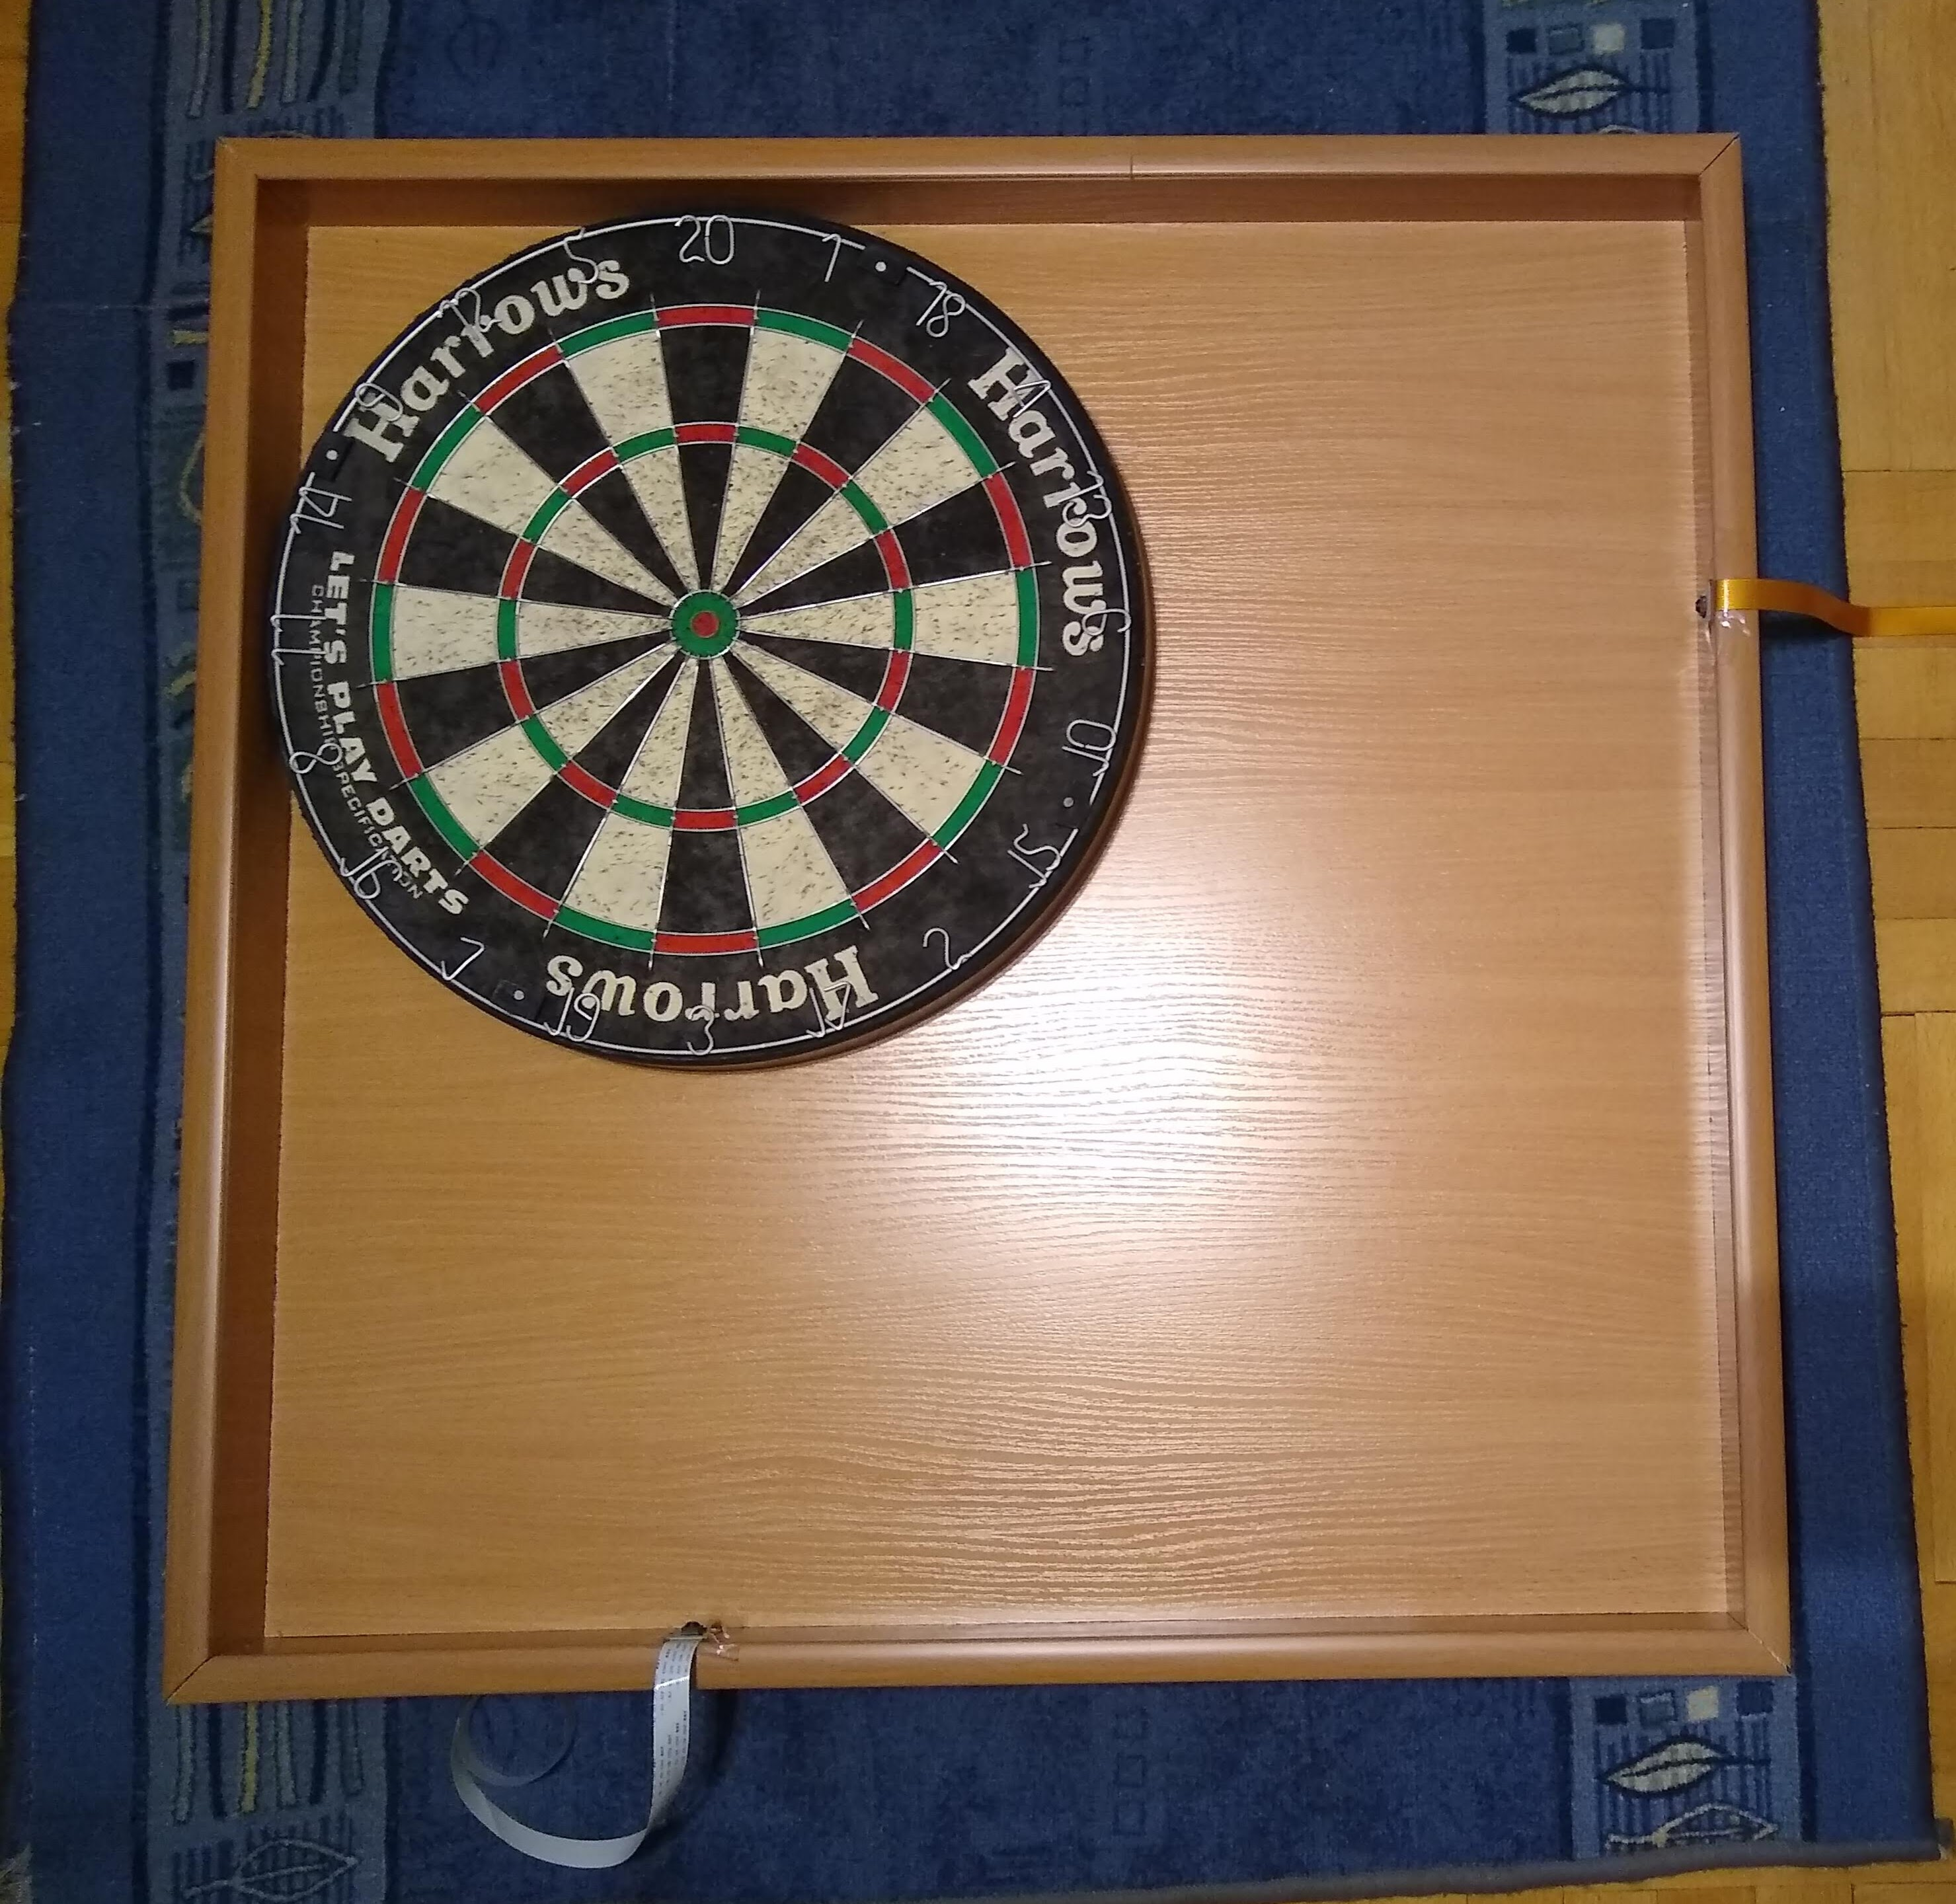
\includegraphics[width=0.5\textwidth]{obrazki/stelaz_live.jpg}
  \captionsource{{\color{dgray}Ukończony stelaż}}{Opracowanie własne}
  \label{stelaz_zdjecie}
\end{subfigure}
\end{figure}

Przed wykonaniem stelaża należało określić, jakie powinien mieć wymiary. Podstawowym warunkiem było to, że kamera musi obejmować cały obszar tarczy, a jednocześnie cały stelaż powinien być jak najmniejszy. Dlatego pierwszym krokiem było odpowiedzenie na pytanie:

\begin{question}
W jakiej minimalnej odległości od środka tarczy w kształcie koła o promieniu $r$ powinna znaleźć się kamera o kącie widzenia $\alpha$, by na zdjęciu cała tarcza była widoczna? 
\end{question}

\begin{figure}[h!]
\begin{center}
\includesvg[width=0.5\textwidth]{obrazki/odleglosc_kamery.svg}
\end{center}
\captionsource{{\color{dgray}Rysunek pomocniczy}}{Opracowanie własne}
\label{odleglosc_kamery}
\end{figure} 

Do przedstawienia rozwiązania pomocny jest rysunek \ref{odleglosc_kamery}. $P$ oznacza środek kamery, $O$ to środek tarczy (początek układu współrzędnych), $d$ to odległość pomiędzy $P$ a $O$. Przyjmuje się, że kamera jest zwrócona dokładnie na wprost tarczy, dlatego odcinek $OP$ jest dwusieczną kąta $APB$. Pole wyznaczone przez półproste $l$ i $m$ to pole widzenia kamery. By cała tarcza była widoczna, koło musi być zawarte w tym polu. Ponieważ zadaniem jest znalezienie minimalnej odległości, wystarczy by proste $l$ i $m$ były styczne do okręgu. \newline

\noindent Kąty:
\begin{gather*}
\measuredangle PAO = \measuredangle PBO = \pi - \frac{\pi}{2} - \frac{\alpha}{2} = \frac{\pi - \alpha}{2} 
\end{gather*}
Równania prostych i okręgu:
\begin{gather*}
l: y = a_1x + b_1 \\
m: y = a_2x + b_2 \\
x^2 + y^2 = r^2
\end{gather*}
Ponieważ współczynnik kierunkowy prostej jest równy tangensowi kąta nachylenia do osi $OX$, otrzymuje się:
\begin{gather*}
a_1 = \tan (\frac{\pi - \alpha}{2}) \\ 
a_2 = \tan (\pi - \frac{\pi - \alpha}{2}) = \tan (\frac{\pi + \alpha}{2})
\end{gather*}
Półproste $l$ i $m$ przecinają się w punkcie $P(0, d)$:
\begin{gather*}
a_1 \cdot 0 + b_1 = a_2 \cdot 0 + b_2 \\
b_1 = b_2 = d
\end{gather*}
Proste przecinają się z osią $OY$ w tym sam punkcie, więc mają ten sam wyraz wolny, równy $d$.
\begin{gather*}
l: y = \tan (\frac{\pi - \alpha}{2})x + d \\
m: y = \tan (\frac{\pi + \alpha}{2})x + d
\end{gather*}
Teraz wystarczy, by następujący układ równań miał jedno rozwiązanie (można by również użyć równania drugiej prostej, nie ma to znaczenia):
\begin{gather*}
x^2 + y^2 = r^2 \\ 
y = \tan (\frac{\pi + \alpha}{2})x + d
\end{gather*}
Podstawienie:
\begin{gather*}
x^2 + (\tan(\frac{\pi + \alpha}{2})x + d)^2 - r^2 = 0 \\
x^2 + \tan^2(\frac{\pi + \alpha}{2})x^2 + 2\tan(\frac{\pi + \alpha}{2})dx + d^2 - r^2 = 0 \\
[\tan^2(\frac{\pi + \alpha}{2}) + 1]x^2 + 2\tan(\frac{\pi + \alpha}{2})dx + d^2 - r^2 = 0
\end{gather*}
To równanie kwadratowe musi mieć dokładnie jedno rozwiązanie, dlatego $\Delta = 0$:
\begin{equation*}
\begin{split}
\Delta & = [2\tan(\frac{\pi + \alpha}{2})d]^2 - 4\cdot[\tan^2(\frac{\pi + \alpha}{2}) + 1]\cdot (d^2 - r^2) = \\
 & = 4\tan^2(\frac{\pi + \alpha}{2})d^2 - 4[\tan^2(\frac{\pi + \alpha}{2})d^2 - \tan^2(\frac{\pi + \alpha}{2})r^2 + d^2 - r^2] = \\
 & = 4[\tan^2(\frac{\pi + \alpha}{2})d^2 - \tan^2(\frac{\pi + \alpha}{2})d^2 + \tan^2(\frac{\pi + \alpha}{2})r^2 - d^2 + r^2] = \\
 & = 4[(\tan^2(\frac{\pi + \alpha}{2}) + 1)r^2 - d^2]
\end{split}
\end{equation*}
\begin{gather*}
\Delta = 0 \\
4[(\tan^2(\frac{\pi + \alpha}{2}) + 1)r^2 - d^2] = 0 \\
(\tan^2(\frac{\pi + \alpha}{2}) + 1)r^2 - d^2 = 0 \\
d^2 = (\tan^2(\frac{\pi + \alpha}{2}) + 1)r^2 \\
d_1 = r\sqrt{\tan^2(\frac{\pi + \alpha}{2}) + 1} \lor d_2 = - r\sqrt{\tan^2(\frac{\pi + \alpha}{2}) + 1}
\end{gather*}
Ponieważ $d > 0$ (z rysunku), to można odrzucić rozwiązanie $d_2$ -- wyrażenie pod pierwiastkiem jest dodatnie (kwadrat zwiększony o jeden), promień również jest dodatni, więc całe $d_2 < 0$. Ostatecznie:
\begin{gather*}
d = r\sqrt{\tan^2(\frac{\pi + \alpha}{2}) + 1}
\end{gather*}
Dla tarczy i kamery użytych w systemie, gdzie $r = 22,5$ cm, a $\alpha = 53,37\degree$, $d = 50,1$ cm.

Na podstawie tej wartości ustalono wymiary całego stelaża. Najmniejsze możliwe wymiary, to $(d + r) \times (d + r)$, czyli $72,6$ cm $\times \ 72,6$ cm. Wykonany stelaż jest nieco większy ($74,5$ cm $\times \ 74,5$ cm), m.in. z powodu uwzględnienia niezerowej grubości kamery oraz pozostawienia zapasu na ewentualne modyfikacje i pomyłki.
% TODO: można dodać info o trzecim wymiarze (wysokości), zarówno w rysunkach, jak i obliczeniach

\begin{gather*}
\end{gather*}

\section{Obliczenia}
% TODO: zmienić tytuł
Zgodnie z wcześniej przedstawioną ideą, rozwiązanie zostało oparte na stworzeniu trójkąta z dwoma znanymi kątami i jednym znanym bokiem, co pozwala później na obliczenie wszystkich boków trójkąta. Zobrazowane jest to na rysunku \ref{stelaz_trojkat}, do którego kolejne części pracy często będą nawiązywać. Wspomnianym trójkątem jest $\triangle ABP$. $A$ i $B$ to położenia kamer, a $P$ to miejsce wbicia rzutki, które jest celem obliczeń. Kąty $\gamma$ i $\delta$ obliczane są na podstawie pozycji pikseli, a odległość pomiędzy kamerami jest znana lub łatwa do obliczenia z twierdzenia Pitagorasa w $\triangle ABC$.

\begin{figure}[h!]
\begin{center}
\includesvg[width=0.5\textwidth]{obrazki/stelaz_trojkat.svg}
\end{center}
\captionsource{{\color{dgray}Szukany trójkąt w układzie stelaża}}{Opracowanie własne}
\label{stelaz_trojkat}
\end{figure} 

Oto etapy obliczeń, składających się na rozwiązanie głównego problemu:
\begin{itemize}
  \item uzyskanie pozycji piksela, który reprezentuje miejsce wbicia rzutki (dla każdej z kamer)
  \item obliczenie (ze współrzędnych piksela) kąta pomiędzy kamerą a rzutką  (dla każdej z kamer)
  \item umiejscowienie kątów w układzie związanym z kamerami, sformułowanie trójkąta kamera-kamera-rzutka
  \item obliczenie nieznanych kątów i boków trójkąta
  \item obliczenie pozycji $(x, y)$ rzutki, a następnie zamiana układu odniesienia na taki, gdzie $(0, 0)$ to środek tarczy
  \item zamiana współrzędnych kartezjańskich na biegunowe
  \item przyporządkowanie współrzędnych biegunowych $(r, \varphi)$ do pola punktowego (segmentu) na tarczy
\end{itemize}

% TODO: sprecyzuj, co to za kąty (te z kamery), bo to co napisałeś, to nie do końca prawda

Pierwszą fazą analizy rzutu jest przetwarzanie obrazu, którego wynikiem są dane o dwóch pikselach, uznanych za miejsce wbicia lotki, po jednym przez każdą z kamer. Jest to trudne zadanie, które zostanie szerzej omówione w następnym rozdziale. 

Obliczenie kąta pomiędzy kamerą a rzutką jest oparte na prostym założeniu, iż kamera liniowo dystrybuuje miejsce na zdjęciu w stosunku do kąta, pod jakim znajduje się punkt. Oznacza to, że piksele wysunięte najbardziej na lewo odpowiadają kątowi zerowemu, najbardziej na prawo -- maksymalnemu kątowi widzenia kamery ($\alpha$), a wszystkie pomiędzy nimi są proporcjonalnie mniejsze lub większe (liniowa interpolacja). Założenie jest dość silne, ponieważ przy niektórych obiektywach, np. typu rybie oko, fragmenty położone przy brzegach obrazu są w innym stopniu powiększone, niż te, które są bliskie środka (dystorsja). W takich przypadkach przyjęcie takiego założenia skutkowałoby dużymi błędami. 

Dla zdjęcia o wymiarach $w \times h$ pikseli, zrobionego przez kamerę o kącie widzenia $\alpha$, na którym rozważany jest piksel o pozycji $(x, y)$, zachodzi proporcja:

$$
\frac{x}{w} = \frac{\beta}{\alpha}
$$ gdzie $\beta$ oznacza kąt od kamery do rzutki. 
% TODO: może zmienić z w na w-1?
Stąd:
$$
\beta = \frac{x \cdot \alpha}{w}
$$
Warto zauważyć, że wartość $y$ nie ma w tej sytuacji znaczenia, wpływ na wynik ma tylko pozycja na osi poziomej. Na rysunku \ref{zdjecie_interpolacja} pokazana jest siatka pikseli z oznaczeniami rzędów i kolumn, wraz z zaznaczonym pojedynczym pikselem. Rysunek \ref{kat_interpolacja} przedstawia, jaką informację udaje się otrzymać na podstawie pozycji owego piksela -- kąt $\beta$.


\begin{figure}[h!]
\centering
\begin{subfigure}{.5\textwidth}
  \centering
  \includesvg[width=.8\linewidth]{obrazki/zdjecie_interpolacja.svg}
  \caption{siatka pikseli}
  \label{zdjecie_interpolacja}
\end{subfigure}%
\begin{subfigure}{.5\textwidth}
  \centering
  \includesvg[width=.6\linewidth]{obrazki/kat_interpolacja.svg}
  \caption{przybliżony kąt}
  \label{kat_interpolacja}
\end{subfigure}
\captionsource{{\color{dgray}Użycie współrzędnych piksela do wyznaczenia kąta}}{Opracowanie własne.}
\end{figure}

Jednak otrzymany kąt $\beta$ nie odpowiada na razie kątom zaznaczonym na rysunku \ref{stelaz_trojkat}. Należy go poddać jeszcze niewielkim transformacjom. 
\begin{align*}
\gamma &=  45\degree - (\beta_A - \frac{\alpha}{2}) \\
\delta &=  45\degree + \beta_B - \frac{\alpha}{2},
\end{align*}
gdzie $\beta_A, \beta_B$ to kąty $\beta$ odpowiednio dla kamery $A$ i $B$.

Aby zrozumieć powyższe przekształcenia, dobrze jest posłużyć się przykładem, gdy punkt $P$ znajduje się dokładnie na środku tarczy. Wtedy trójkąt $ABP$ jest równoramiennym trójkątem prostokątnym, a więc $\gamma = \delta = 45\degree$, lecz $\beta_A = \beta_B = \frac{\alpha}{2}$. Należy przyjąć tę sytuację jako sytuację wyjściową do kolejnych obliczeń. Dlatego pierwszym krokiem jest zmiana zbioru wartości, które przyjmuje $\beta$: zakres, zamiast od $0$ do $\alpha$, powinien wynosić od $-\frac{\alpha}{2}$ do $\frac{\alpha}{2}$. Ta zmiana dokonuje się przez odjęcie od wyliczonego kąta wartości $\frac{\alpha}{2}$. Jest to teraz kąt nie od lewego ramienia do prostej przecinającej punkt $P$, lecz od prostej biegnącej przez środek obrazu do prostej przecinającej punkt $P$. Dzięki temu, dla punktu z przykładu, kąt wynosi $0\degree$, ponieważ znajduje się dokładnie na wprost kamery. Kolejną zależnością, którą należy uwzględnić, jest fakt, iż im większy jest kąt $\beta_A$, tym mniejszy jest kąt $\gamma$. Stąd wynika konieczność zmiany znaku kąta dla kamery $A$, przez co pierwszy (licząc od lewej) piksel będzie oznaczał kąt $\frac{\alpha}{2}$, a ostatni $-\frac{\alpha}{2}$ (a nie odwrotnie). Dla kamery $B$ nie ma potrzeby takiej zamiany: im większy kąt $\beta_B$, tym większy kąt $\delta$. Po przedstawionych transformacjach należy dodać jeszcze $45 \degree$, tak by punkt znajdujący się na wprost kamery był ostatecznie interpretowany jako $45 \degree$.

Dzięki powyższym obliczeniom, dostępne są wszystkie dane potrzebne do jednoznacznego wyznaczenia trójkąta $ABP$. Jego trzeci kąt można obliczyć, korzystając z własności, że suma kątów w trójkącie wynosi $180\degree$:
$$
\measuredangle APB = \varepsilon = 180\degree - \gamma - \delta
$$
Długości boków uzyskuje się za pomocą twierdzenia sinusów:
\begin{gather*}
\frac{|AB|}{\sin\varepsilon} = \frac{|BP|}{\sin\gamma} = \frac{|AP|}{\sin\delta} \\[1em]
|BP| = \frac{|AB| \cdot \sin\gamma}{\sin\varepsilon} \\[1em]
|AP| = \frac{|AB| \cdot \sin\delta}{\sin\varepsilon}
\end{gather*}

Na podstawie danych o trójkącie $ABP$, należy obliczyć pozycję punktu $P$, umieszczając trójkąt w układzie współrzędnych, w którym punkt $A$ jest początkiem. Szkic pomocniczy znajduje się na rysunku \ref{trojkat_kartezjanskie}. Pozycja punktu B jest określona przy tworzeniu stelaża -- najczęściej będzie to $(d, d)$, jednak w poniższych obliczeniach zakłada się ogólniejszy przypadek, gdzie współrzędne punktu na obu osiach nie muszą się sobie równać. Przyjęto oznaczenie $B(w, h)$. Jedynymi szukanymi w tym podproblemie są $x$ oraz $y$, czyli współrzędne punktu $P$. Obliczenia opierają się na działaniach wektorowych: wyznacza się wektor $\overrightarrow{AP} = \overrightarrow{b}$ oraz $\overrightarrow{AB} = \overrightarrow{a}$.

\begin{figure}[h!]
\begin{center}
\includesvg[width=0.5\textwidth]{obrazki/trojkat_kartezjanskie.svg}
\end{center}
\captionsource{{\color{dgray}Układ współrzędnych o środku w $A$}}{Opracowanie własne}
\label{trojkat_kartezjanskie}
\end{figure} 

Główne równanie wynika z wzoru na kąt między wektorami:
\begin{gather*}
\cos \gamma = \frac{\vec{a}\circ\vec{b}}{|\vec{a}|\cdot |\vec{b}|} = \frac{[w, h]\circ[x, y]}{|\vec{a}|\cdot |\vec{b}|} = \frac{wx + hy}{|\vec{a}|\cdot |\vec{b}|} \\[1em]
|\vec{a}|\cdot |\vec{b}| \cos \gamma = wx + hy \\[1em]
x = \frac{|\vec{a}|\cdot |\vec{b}| \cos \gamma - hy}{w}
\end{gather*}
Drugą zależnością, z której należy skorzystać, jest wzór na długość wektora:
\begin{align*}
|\vec{b}| &= \sqrt{x^2 + y^2} \\
|\vec{b}|^2 &= x^2 + y^2
\end{align*}
Podstawienie:
\begin{align*}
|\vec{b}|^2 &= \left(\frac{|\vec{a}|\cdot |\vec{b}| \cos \gamma - hy}{w}\right)^2 + y^2 \\ 
|\vec{b}|^2 &= \frac{(|\vec{a}|\cdot |\vec{b}| \cos \gamma - hy)^2}{w^2} + y^2 \\ 
|\vec{b}|^2 &= \frac{1}{w^2}\left(|\vec{a}|^2\cdot |\vec{b}|^2 \cos^2 \gamma - 2|\vec{a}|\cdot |\vec{b}|h \cos \gamma\ y + h^2 y^2\right) + y^2 \\ 
|\vec{b}|^2 &= \frac{1}{w^2}|\vec{a}|^2\cdot |\vec{b}|^2 \cos^2 \gamma - \frac{2}{w^2}|\vec{a}|\cdot |\vec{b}|h \cos \gamma\ y + \left(1 + \frac{h^2}{w^2}\right) y^2 \\
\bigg(1 &+ \frac{h^2}{w^2}\bigg)  y^2 - \frac{2}{w^2}|\vec{a}|\cdot |\vec{b}|h \cos \gamma\ y + |\vec{b}|^2\left(\frac{|\vec{a}|^2 \cos^2 \gamma}{w^2} - 1 \right) = 0
\end{align*}
Otrzymano równanie kwadratowe postaci $a_2y^2 + a_1y + a_0$, gdzie:
\begin{align*}
a_2 &= 1 + \frac{h^2}{w^2} \\
a_1 &= -\frac{2}{w^2}|\vec{a}|\cdot |\vec{b}|h \cos \gamma \\
a_0 &= |\vec{b}|^2\left(\frac{|\vec{a}|^2 \cos^2 \gamma}{w^2} - 1 \right)
\end{align*}
Wzory na pierwiastki tego równania nie są podawane, ponieważ również w implementacji korzysta się z zewnętrznej biblioteki do wyliczania pierwiastków, odpornej na błędy numeryczne. W przypadku, gdy równanie ma dwa rozwiązania, wybierane jest $y >0$.

Pierwsza współrzędna obliczana z wcześniej już przedstawionego wzoru:
$$
x = \frac{|\vec{a}|\cdot |\vec{b}| \cos \gamma - hy}{w}
$$

Następnie należy przenieść układ współrzędnych w taki sposób, by jego początkiem był środek tarczy. Przekształceniem, które to zapewnia, jest funkcja $f$:
$$
f(x, y) = (x, y + h)
$$

W celu łatwiejszego przyporządkowania pozycji rzutki do pola na tarczy, warto przedstawić ją za pomocą współrzędnych biegunowych, tzn. promienia $r_p$ od środka tarczy ($O$) do punktu $P$ oraz kąta $\varphi$ pomiędzy półprostą $OB$ a wektorem $\overrightarrow{OP}$. \newline
Promień $r_p$ wyliczany jest ze wzoru na długość wektora (z tw. Pitagorasa):
$$
r_p = \sqrt{x^2 + y^2}
$$
Wzór na wartość kąta $\varphi$ jest zależny od ćwiartki układu, w jakiej znajduje się punkt:
$$
\varphi = 
     \begin{cases}
       arctg(\frac{y}{x}) &\quad\text{gdy } x > 0 \land y \ge 0 \\
       arctg(\frac{y}{x}) + 2\pi &\quad\text{gdy } x > 0 \land y < 0 \\
       arctg(\frac{y}{x})+ \pi &\quad\text{gdy } x < 0 \\
       \frac{\pi}{2} &\quad\text{gdy } x = 0 \land y > 0 \\ 
       \frac{3\pi}{2} &\quad\text{gdy } x = 0 \land y < 0
     \end{cases}
$$

Ostatnim etapem jest przypisanie współrzędnym biegunowym konkretnego pola na tarczy. Patrząc na kołową budowę tarczy łatwo zauważyć, że kąt $\varphi$ wskazuje, w który wycinek kołowy trafiła rzutka, a promień $r_p$ pozwala określić, czy jest to pole standardowe, podwójne, potrójne itd. Do reprezentacji segmentu będzie używana notacja z sekcji \ref{reprezentacja_pola}.
	\cleardoublepage
	
	\chapter{Projekt systemu}
\thispagestyle{chapterBeginStyle}

Niniejszy rozdział traktuje o procesach systemu, jego składowych i powiązaniach między nimi. Do ich przedstawienia używane są opisy słowne oraz diagramy UML. Istotnym elementem jest prezentacja sposobu, w jaki przetwarzane są obrazy w systemie oraz algorytmów z tym związanych.

\section{Przypadki użycia}
Powiązany z systemem jest obecnie jeden, główny przypadek użycia. Aktorem jest gracz, który po uruchomieniu aplikacji mobilnej łączy się z systemem wbudowanym podłączonym do tarczy. Po informacji o ustanowieniu połączenia, może on zacząć wykonywać rzuty. Po każdym rzucie, w krótkim czasie, otrzymuje on informację o polu, w jakie trafił oraz wizualizację miejsca wbicia lotki na graficznym schemacie tarczy. Aplikacja, w razie potrzeby, sygnalizuje problemy z połączeniem na linii klient-serwer.

\section{Urządzenia i komponenty}
W systemie występują następujące urządzenia:
\begin{itemize}
  \item minikomputer \verb|Raspberry Pi 4 B|;
  \item minikomputer \verb|Raspberry Pi Zero W|;
  \item dwie kamery \verb|Camera Module v1 (OmniVision OV5647)|;
  \item smartfon.
\end{itemize}

Na diagramie wdrożenia (\ref{deployment}) pokazano te urządzenia wraz z połączeniami między nimi oraz komponentami, jakie wchodzą w ich skład. \verb|Raspberry Pi 4| jest najważniejszym urządzeniem, które synchronizuje pracę innych oraz dokonuje obliczeń. Łączy się z kamerą za pomocą kabla taśmowego, a używa jej do wykrywania rzutu za pomocą biblioteki \verb|OpenCV|. Analogicznie wygląda to w przypadku \verb|Pi Zero|, na którym znajduje się druga instancja detektora rzutu. Informacje wysyłane są z \verb|Pi Zero| do \verb|Pi 4| z użyciem gniazd TCP. Na \verb|Pi 4| tworzony jest również serwer dla aplikacji mobilnej, która uruchamiana jest na smartfonie w środowisku Expo \cite{expo}. Połączenie następuje zgodnie ze standardem WebSocket.

% TODO: może inna czcionka w UML?
\begin{figure}[h!]
\begin{center}
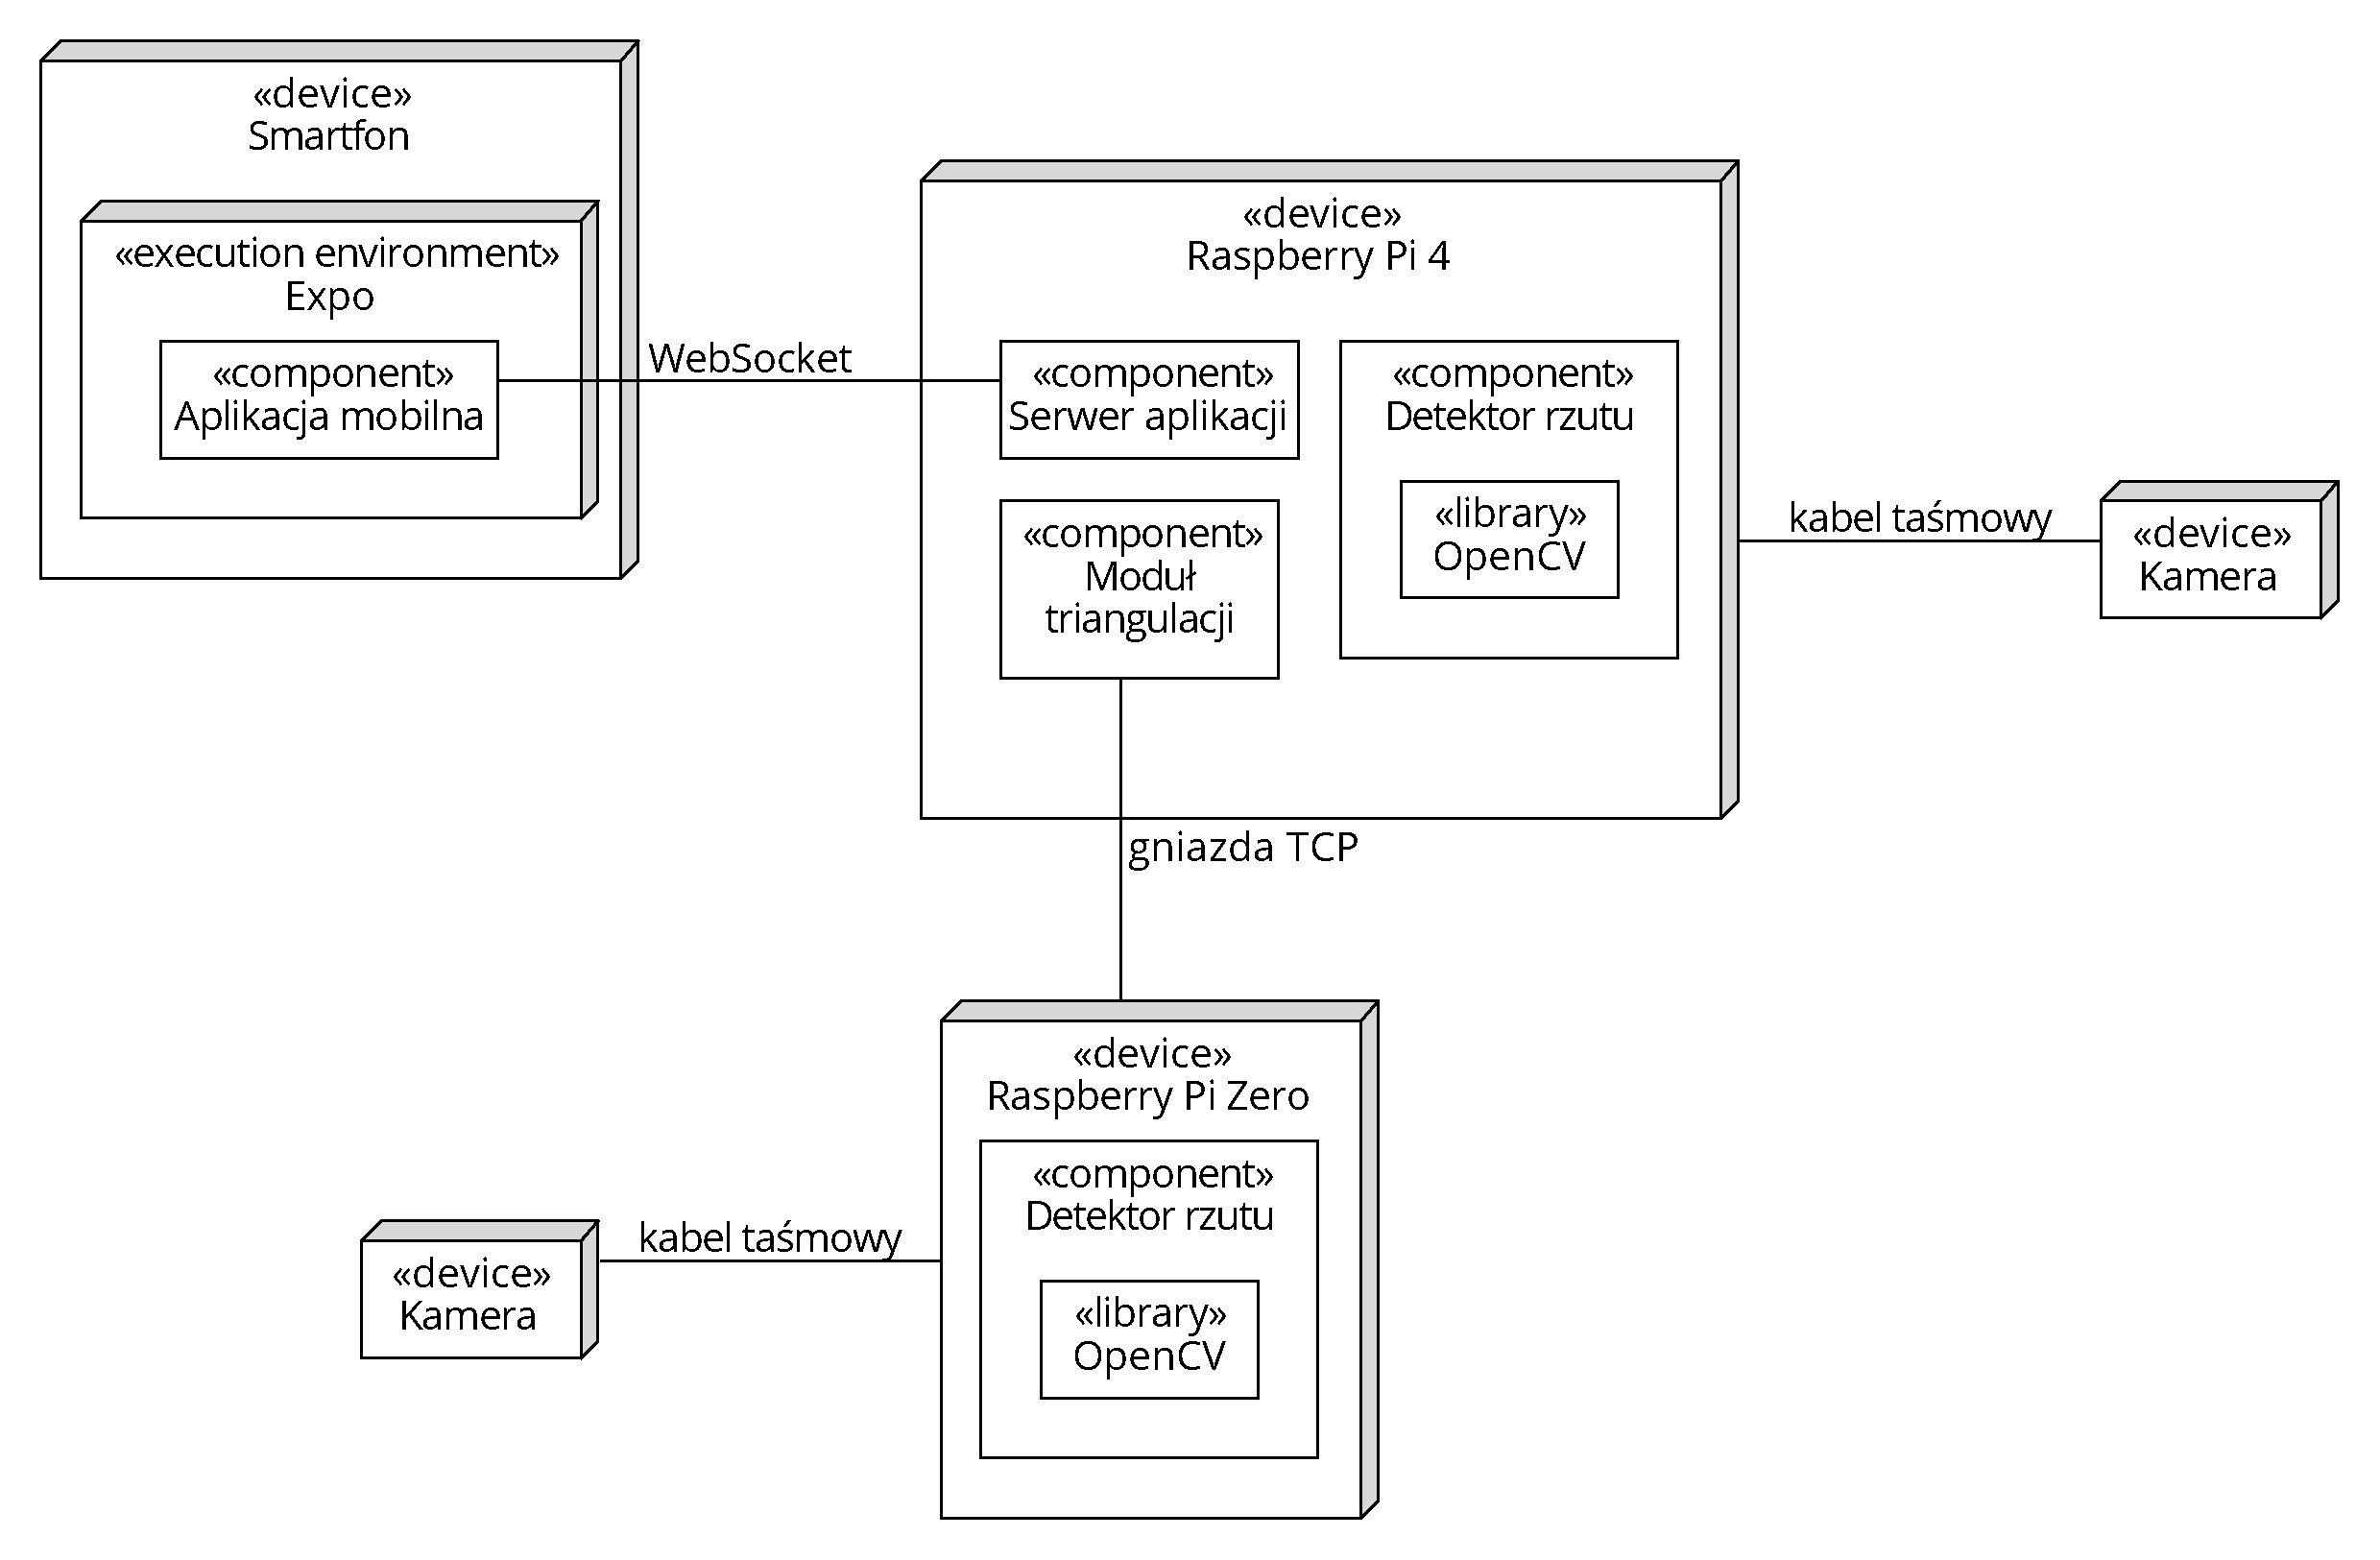
\includegraphics[width=\textwidth]{obrazki/deployment.pdf}
\end{center}
\captionsource{{\color{dgray}Diagram wdrożeniowy}}{Opracowanie własne}
\label{deployment}
\end{figure}

\section{Diagramy aktywności}
Na diagramie aktywności (\ref{activity}) przedstawiono logikę procesu zachodzącego w systemie z zachowaniem wysokiego poziomu ogólności. System rozpoczyna działanie od rozwidlenia na przetwarzanie obrazu z użyciem kamery dolnej oraz prawej. W obu przypadkach wygląda to identycznie - w pętli wykonywane są zdjęcia i poddawane analizie. W przypadku wykrycia rzutu pętla zostaje przerwana, a program synchronizuje się z drugą kamerą i przeprowadza obliczenia prowadzące do pozycji rzutki, która zostaje wyświetlona w aplikacji mobilnej. Następnie proces rozpoczyna się od początku.

\begin{figure}[h!]
\begin{center}
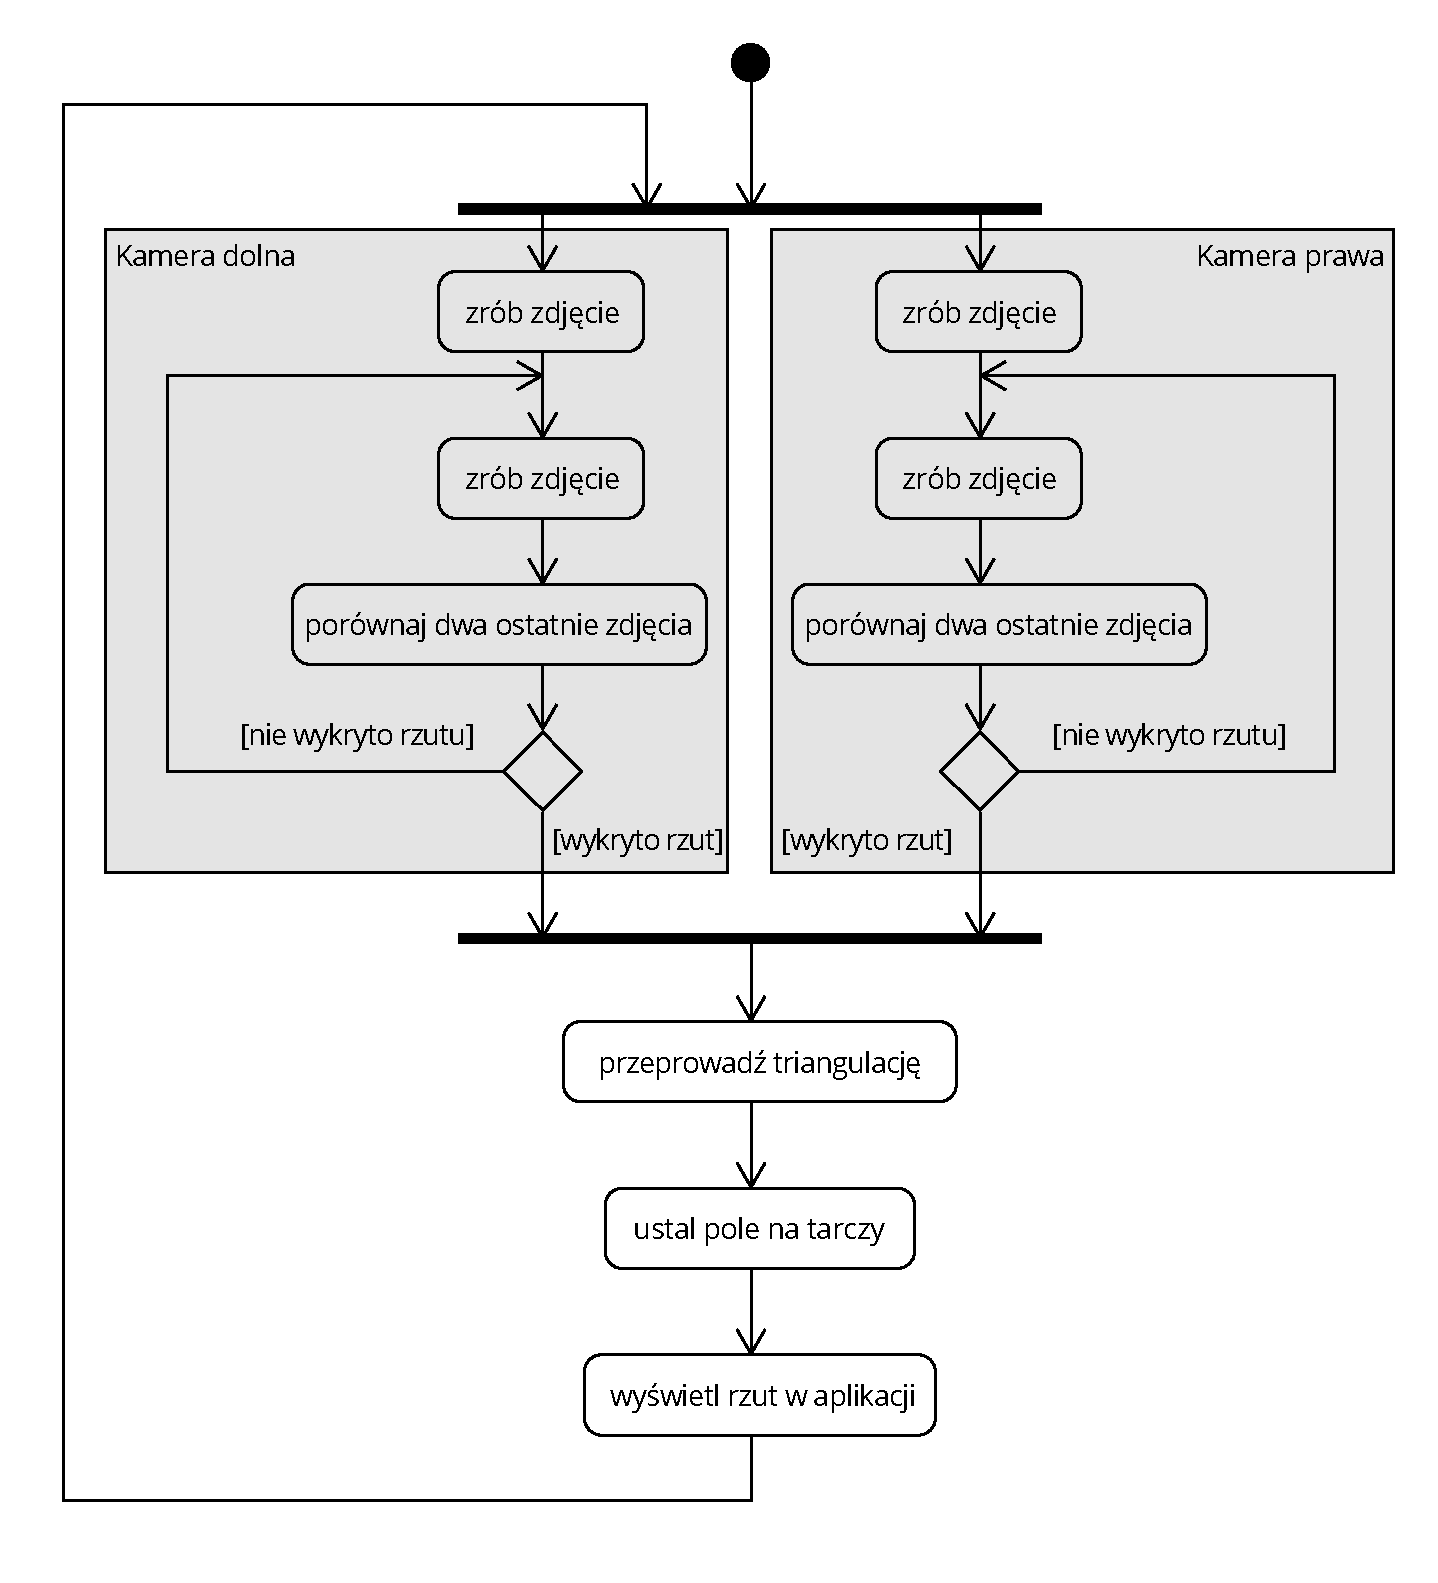
\includegraphics[width=\textwidth]{obrazki/activity.pdf}
\end{center}
\captionsource{{\color{dgray}Diagram aktywności}}{Opracowanie własne}
\label{activity}
\end{figure} 

\section{Diagramy sekwencji}
Diagram sekwencji (\ref{sequence}) pokazuje, w jaki sposób odbywa się komunikacja pomiędzy poszczególnymi komponentami. Jako pierwszy startuje program na \verb|Raspberry Pi 4|. Najpierw czeka on na połączenie z drugim minikomputerem, \verb|Pi Zero| oraz w osobnym wątku tworzy serwer dla aplikacji mobilnej. Gracz może wtedy włączyć aplikację, która natychmiastowo połączy się z tymże serwerem. W tym momencie gracz może zacząć wykonywanie rzutów. \verb|Pi 4| oraz \verb|Pi Zero| równolegle wykrywają rzut, lecz po wykryciu rzutu przez pierwszego z nich, czeka on na dane o położeniu piksela, nadchodzące z drugiego. Później, po przeprowadzeniu obliczeń, informacje o rzucie są przesyłane od serwera do aplikacji mobilnej. Możliwe jest podłączenie wielu klientów -- serwer posiada listę podłączonych użytkowników i wysyła informacje do każdego z nich. 
\begin{figure}[h!]
\begin{center}
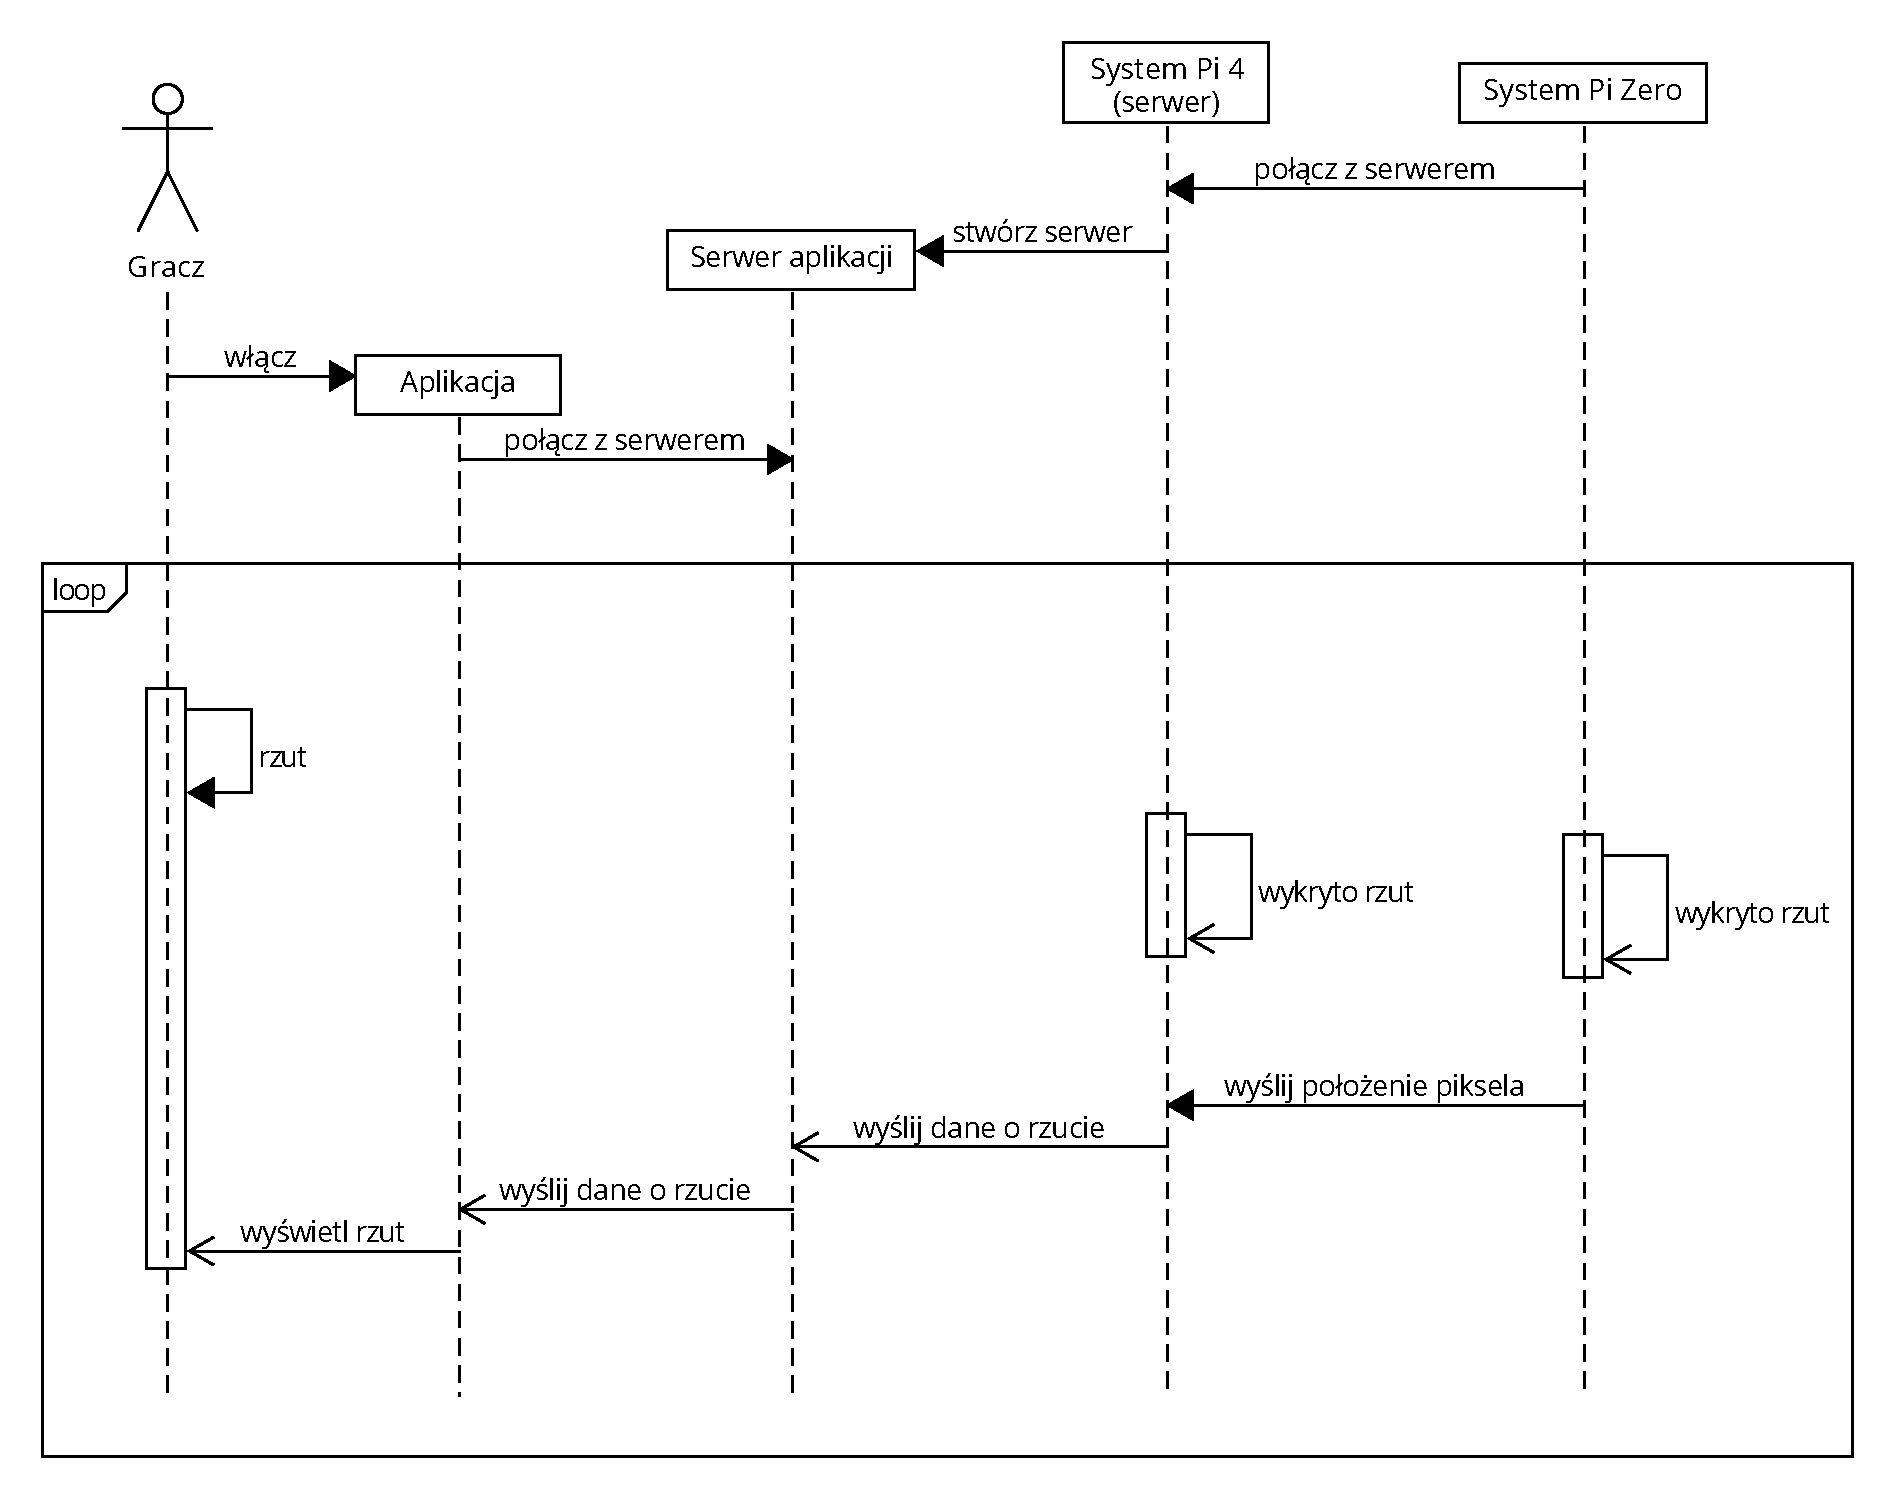
\includegraphics[width=\textwidth]{obrazki/sequence.pdf}
\end{center}
\captionsource{{\color{dgray}Diagram sekwencji}}{Opracowanie własne}
\label{sequence}
\end{figure}

\section{Opis protokołów}
W systemie do komunikacji używa się dwóch protokołów: TCP \cite{TCP} i WebSocket \cite{WebSocket}. Pierwszy z nich używany jest do wysłania informacji z \verb|Pi Zero| do \verb|Pi 4| w sposób binarny: 3 liczby całkowite (pozycja $x$, pozycja $y$ oraz liczba porządkowa rzutki), po 4 bajty na liczbę, w formacie \textit{big endian}. Drugi protokół stosuje się przy przekazaniu komunikatu o wyliczonej pozycji rzutki. Jego treść jest w formacie \verb|JSON| i została pokazana na listingu \ref{json}. 

\begin{listing}[h!]
\begin{minted}[frame=single,
               framesep=3mm,
               linenos=true,
               xleftmargin=21pt,
               tabsize=4]{js}
{     
    "x": 23.123516,
    "y" : 5.7825,
    "segment" : 20
}
\end{minted}
\caption{Przykładowy komunikat o wykrytej rzutce} 
\label{json}
\end{listing}

\section{Algorytm przetwarzania obrazu}
Podstawowym algorytmem, który nie został opisany w poprzednim rozdziale, jest proces przetwarzania obrazu. Zadaniem, które należy wykonać za pomocą metod związanych z tą dziedziną, jest odjęcie tła (ang. \textit{background substraction}). Polega ono na wyodrębnieniu elementów pojawiających się na pierwszym planie, na podstawie następujących po sobie zdjęć. W prezentowanym systemie użyte zostało w celu wykrycia rzutu, a następnie ustalenia samej pozycji rzutki na zdjęciu. W ogólności jest to zadanie trudne, ze względu na możliwe zmiany tła, spowodowane m.in. minimalnym ruchem lub zmianą warunków oświetlenia. Podejść do jego rozwiązania jest wiele \cite{LearningOpenCV}, jednak w niniejszej pracy, z powodu niewielkiej liczby tego typu czynników, zastosowano jedno z najprostszych - odejmowanie od siebie dwóch kolejnych klatek.

Każda z kamer, co pewien krótki czas, wykonuje zdjęcie. Następnie, dwa ostatnie zdjęcia z danej kamery, są od siebie odejmowane. Dzięki reprezentacji macierzowej, działanie to odbywa się zgodnie z zasadami bezwzględnego odejmowania macierzy. Jego wynikiem jest nowe zdjęcie, w której piksele niezmienione w czasie pomiędzy wykonaniem klatek powinny być bliskie wartości 0 (piksel czarny), zaś te reprezentujące pojawienie się nowego obiektu -- wyraźnie większe od zera. Aby zmniejszyć występujące szumy oraz przekształcić obraz na binarny (czarno-biały), stosuje się następnie funkcję progową (ang. \textit{threshold}), która wszystkie piksele o wartościach niższych od ustalonego progu zamienia na czarne, a wyższe -- na piksele białe. 

Tak przygotowane zdjęcie należy poddać wykrywaniu konturów. Konturem nazywa się zbiór punktów reprezentujących krzywą \cite{LearningOpenCV}. W przypadku problemu omawianego w pracy, celem jest wykrycie konturu wokół rzutki, która pojawiła się na ostatnio wykonanym zdjęciu. % TODO: opisz findContours()
Algorytm wykrywania konturów jest dość skomplikowany, jego szczegóły można znaleźć w pracach Suzuki \cite{ContoursAlgorithm}. Po uzyskaniu listy konturów wybierany jest największy z nich (pod względem powierzchni, którą wyznacza), a następny poddany analizie, czy jest to kontur rzutki. Należy wyznaczyć charakterystyczne cechy lotki na zdjęciu, opierając się na empirycznych danych pochodzących z testów. W obecnej implementacji kontur jest uznawany za kontur rzutki wtedy, gdy powierzchnia przez niego wyznaczona mieści się w określonych doświadczalnie granicach. Innymi sposobami jest na przykład sprawdzanie proporcji długości do szerokości w prostokącie okalającym kontur.  Jeśli nie wykryto żadnych konturów lub nie spełniają one warunków, uznaje się, że rzut nie wystąpił pomiędzy badanymi ujęciami.

Ostatnią fazą jest wybranie pojedynczego piksela, którego pozycja będzie reprezentować miejsce wbicia rzutki: jest to najniżej położony piksel konturu (znajdujący się najbliżej tarczy).
	\cleardoublepage
	
	\chapter{Implementacja systemu}
\thispagestyle{chapterBeginStyle}

W tym rozdziale opisane są szczegóły implementacyjne projektu. Więcej uwagi poświęcono urządzeniom wchodzącym w skład systemu oraz opisano użyte technologie, wraz z uargumentowaniem, dlaczego to właśnie one zostały wybrane. Kolejnym elementem jest omówienie struktury projektu oraz wypunktowania, co znajduje się w poszczególnych plikach z kodem źródłowym. Zaprezentowano na przykładzie wynik działania systemu, opisano problemy napotkane w trakcie pracy oraz przedstawiono sposób prowadzenia projektu.

\section{Opis urządzeń}

\subsection{Raspberry Pi}
Programy wykonywane są na urządzeniach z rodziny Raspberry Pi \cite{RPi}. Są to jednopłytkowe minikomputery, tzw. SoC (ang. \textit{System-on-a-chip}). Ich jednostką obliczeniową jest procesor firmy Broadcom, wykonany w architekturze ARM. Pozwalają na obsługę i komunikację z innymi urządzeniami za pomocą wielu portów i interfejsów: m.in. USB, HDMI, GPIO (40 pinów wejścia/wyjścia ogólnego przeznaczenia), CSI (interfejs kamery), RJ-45, Wi-Fi czy Bluetooth. Nie posiadają one wbudowanej pamięci, wszystkie dane są zapisywane na karcie SD, na której znajduje się również system operacyjny, najczęściej Linux. Organizacja produkująca minikomputery wydaje swoją dystrybucję nazwaną Raspberry Pi OS (wcześniej Raspbian), opartą na Debianie. Wydanych zostało kilka wersji Raspberry różniących się od siebie przeznaczeniem i specyfikacją. W systemie użyto \verb|Pi 4| i \verb|Pi Zero|. Pierwsza z nich to najnowsza wersja, z czterordzeniowym procesorem taktowanym zegarem 1,5 GHz oraz pamięcią RAM 2 GB. Druga zaś jest odpowiedzią na sytuacje, gdzie tak duże moce obliczeniowe nie są potrzebne -- Pi Zero ma mniejsze wymiary, słabszy procesor oraz mniej pamięci RAM, co skutkuje również mniejszą ceną.
\subsection{Kamery}
Kamery użyte w systemie to kamery dedykowane do Raspberry Pi: Camera Module v1 z matrycą OmniVision OV5647. Pozwalają na wykonywanie zdjęć w rozdzielczości 2592 $\times$ 1944 pikseli, ich poziome pole widzenia to $53,5 \degree \pm 0,13 \degree$, a ogniskowa wynosi 3,60 mm. Pełna specyfikacja jest dostępna na stronie producenta \cite{RPi}.

Początkowo planowano użycie jedynie jednego minikomputera, do którego podłączone byłyby dwie kamery USB lub jedna kamera Pi i jedna USB. Pierwszy wariant został odrzucony z powodu wysokiej ceny (lub gorszej jakości) kamer internetowych oraz możliwymi problemami z przepustowością USB. Drugi za to wprowadzałby niepotrzebny brak spójności oraz niemożność reużywania kodu źródłowego, obsługującego kamerę dedykowaną. Dodatkowo, tego typu kamera posiada sprzętowe i programowe wsparcie i oferuje pełną kompatybilność z urządzeniem, co wpływa na szybkość i niezawodność działania. Niemożliwe jest jednak bezpośrednie podłączenie dwóch takich kamer, gdyż \verb|Pi 4| posiada jedynie jeden port CSI. Dlatego zdecydowano się na użycie drugiego, tańszego urządzenia z serii Raspberry, do którego można podłączyć drugą kamerę. 
\clearpage
\section{Technologie}
Użyte technologie:
\begin{itemize}
  \item Python 3.7
  \item OpenCV 4.1.0
  \item picamera 1.13
  \item WebSocket
  \item JavaScript ES6
  \item React Native 0.63
  \item Expo 39
\end{itemize}

Kod źródłowy uruchamiany na obu urządzeniach Raspberry został napisany w języku Python 3.7. Został on wybrany z powodu jego prostoty oraz istnienia wielu bibliotek specyficznych dla minikomputera, które napisane są właśnie w tym języku. Wspiera on wiele paradygmatów programowania, dzięki czemu programista ma swobodę w wyborze sposobu implementacji rozwiązań. Automatyczne zarządzanie pamięcią zmniejsza ryzyko błędów, a sprawdzone biblioteki do operacji macierzowych zapewniają szybkość działania.

Do przetwarzania obrazu użyto biblioteki OpenCV, która dostarcza wiele gotowych modułów do rozwiązywania najczęstszych problemów związanych z widzeniem komputerowym, zapewniając jednocześnie duże możliwości konfiguracji, poprzez dobieranie parametrów. Biblioteka napisana jest w języku C++, ale posiada nakładki pozwalające na wywoływanie funkcji z poziomu innych języków, m.in. Pythona.

Wykonywanie zdjęć za pomocą kamery dedykowanej do Raspberry Pi byłoby trudne bez interfejsu, który dostarcza metody umożliwiające kontrolę pracy kamery na wysokim poziomie abstrakcji, bez wnikania w szczegóły jej budowy. Rolę tego interfejsu pełni picamera \cite{picamera}, moduł napisany w Pythonie specjalnie do tego celu. Pomimo prostoty użytkowania, daje możliwość zmiany wielu parametrów wpływających na zdjęcie, takich jak: czas naświetlania, liczba klatek na sekundę, rozdzielczość czy balans bieli. Dokumentacja opisuje sposób na przekształcenie zdjęć do formatu zgodnego z wymaganiami OpenCV.

Komunikacja pomiędzy serwerem a aplikacją mobilną odbywa się z użyciem protokołu WebSocket. Po stronie aplikacji wsparcie dla tego sposobu komunikacji jest wbudowane, lecz w języku Python należy wybrać jedną z szeregu zewnętrznych bibliotek, w których można stworzyć serwer. Implementacja została oparta o niewielką i mało popularną bibliotekę SimpleWebSocketServer \cite{SimpleWebSocket}, która jest jednak wystarczająca do obecnych potrzeb. 

Do wykonania aplikacji klienckiej użyto platformy programistycznej React Native \cite{ReactNative}, dzięki której za pomocą jednej wersji kodu źródłowego tworzy się aplikację kompatybilną zarówno z systemem Android, jak i iOS. Z powodu bardzo dużych podobieństw do biblioteki React.js i używania języka JavaScript, tworzenie oprogramowania jest bardzo podobne do tworzenia aplikacji webowej. Środowisko Expo \cite{expo} zapewnia za to narzędzia pomocne w rozwijaniu, budowaniu i uruchamianiu aplikacji. Dzięki niemu możliwe jest używanie aplikacji mobilnej również przez przeglądarkę internetową. Wieloplatormowość to zdecydowany atut aplikacji.

\section{Struktura projektu}
\begin{forest}
for tree={font=\sffamily, grow'=0,
folder indent=.9em, folder icons,
edge=densely dotted}
[pi-darts
  [app
      [src
          [assets
              [dartboard.svg, is file]]
          [components
              [Dartboard.js, is file]]
          [helpers
              [WebSocketClient.js, is file]]
          [App.js, is file]]
      [app.json, is file]
      [package.json, is file]]
  [rpi
      [src
          [main$\_$pi4.py, is file]
          [main$\_$pi0.py, is file]
          [app$\_$connector.py, is file]
          [pi$\_$connector.py, is file]
          [camera.py, is file]
          [throw$\_$detector.py, is file]
          [triangulation.py, is file]
          [board$\_$mapping.py, is file]]
      [sync.sh, is file]
      [requirements.txt, is file]]
]
\end{forest}

Folder z projektem o nazwie \verb|pi-darts| zawiera dwie aplikacje: \verb|app| i \verb|rpi|. Pierwsza z nich jest jest uruchamiana na smartfonie, druga na \verb|Pi 4| i \verb|Pi 0|.

\subsubsection{Opis plików źródłowych}
\begin{itemize}
  \item \verb|main_pi4.py| -- główny skrypt uruchamiany na \verb|Pi 4|, konfiguruje pozostałe moduły i zawiera główną pętlę programu.
  \item \verb|main_pi0.py| -- główny skrypt uruchamiany na \verb|Pi Zero|, bardzo podobny do \verb|main_pi4.py|. Również zawiera pętlę, w której wykonywane są nieustannie zdjęcia, lecz nie zajmuje się komunikacją z aplikacją.
  \item \verb|app_connector.py| -- zawiera klasę serwera aplikacji, dostarcza interfejs do wystartowania serwera w osobnym wątku oraz wysyłania komunikatów do klientów.
  \item \verb|pi_connector.py| -- używany przez oba urządzenia w celu ustanowienia połączenia. Składa się z dwóch klas: jednej dla serwera (\verb|Pi 4|), z metodami do uruchomienia gniazda TCP i przyjęcia wiadomości, a drugiej dla klienta (\verb|Pi Zero|), z funkcjami do podłączenia się do serwera oraz wysłania komunikatu.
  \item \verb|camera.py| -- dodatkowy interfejs opakowujący metody biblioteki \verb|picamera|. Daje możliwość wstępnego ustawienia kamery oraz wykonania zdjęcia reprezentowanego w formacie zgodnym z OpenCV.
  \item \verb|throw_detector.py| -- moduł, w którym zaimplementowana jest logika wykrywania rzutu. W tym miejscu wykonywane są wszystkie operacje na obrazach.
  \item \verb|triangulation.py| -- plik, w którym zapisane są funkcje przeprowadzające triangulację
  \item \verb|board_mapping.py| -- komponent przyporządkowujący pozycję rzutki we współrzędnych kartezjańskich do konkretnego pola na rzutce
  \item \verb|App.js| -- główny komponent aplikacji mobilnej. Zarządza jej stanem oraz przekazuje informacje do \verb|Dartboard.js|.
  \item \verb|Dartboard.js| -- komponent ze graficznym przedstawieniem tarczy, umożliwia zaznaczanie miejsca wbicia rzutki.
  \item \verb|WebSocketClient.js| -- pomocniczy plik ustanawiający połączenie oraz przyjmujący komunikaty z serwera za pomocą technologii WebSocket.
  
\end{itemize}

\section{Efekt końcowy}
Efekty działania aplikacji zostaną pokazane na przykładzie. Na rysunku \ref{rzutka_gora} widoczny jest rzut z góry na tarczę z wbitą rzutką w pole standardowe 10. Następnie, na rysunku \ref{rzutka_kontury} zielonym kolorem zaznaczone zostały kontury wokół rzutki, osobno dla każdej z kamer. Pojedynczy, czerwony punkt jest uznawany za miejsce wbicia lotki. Ostateczny rezultat działania systemu widoczny jest na zrzucie ekranu z aplikacji mobilnej, gdzie prezentowane dane dobrze odzwierciedlają wykonany rzut.
\begin{figure}[h!]
\begin{center}
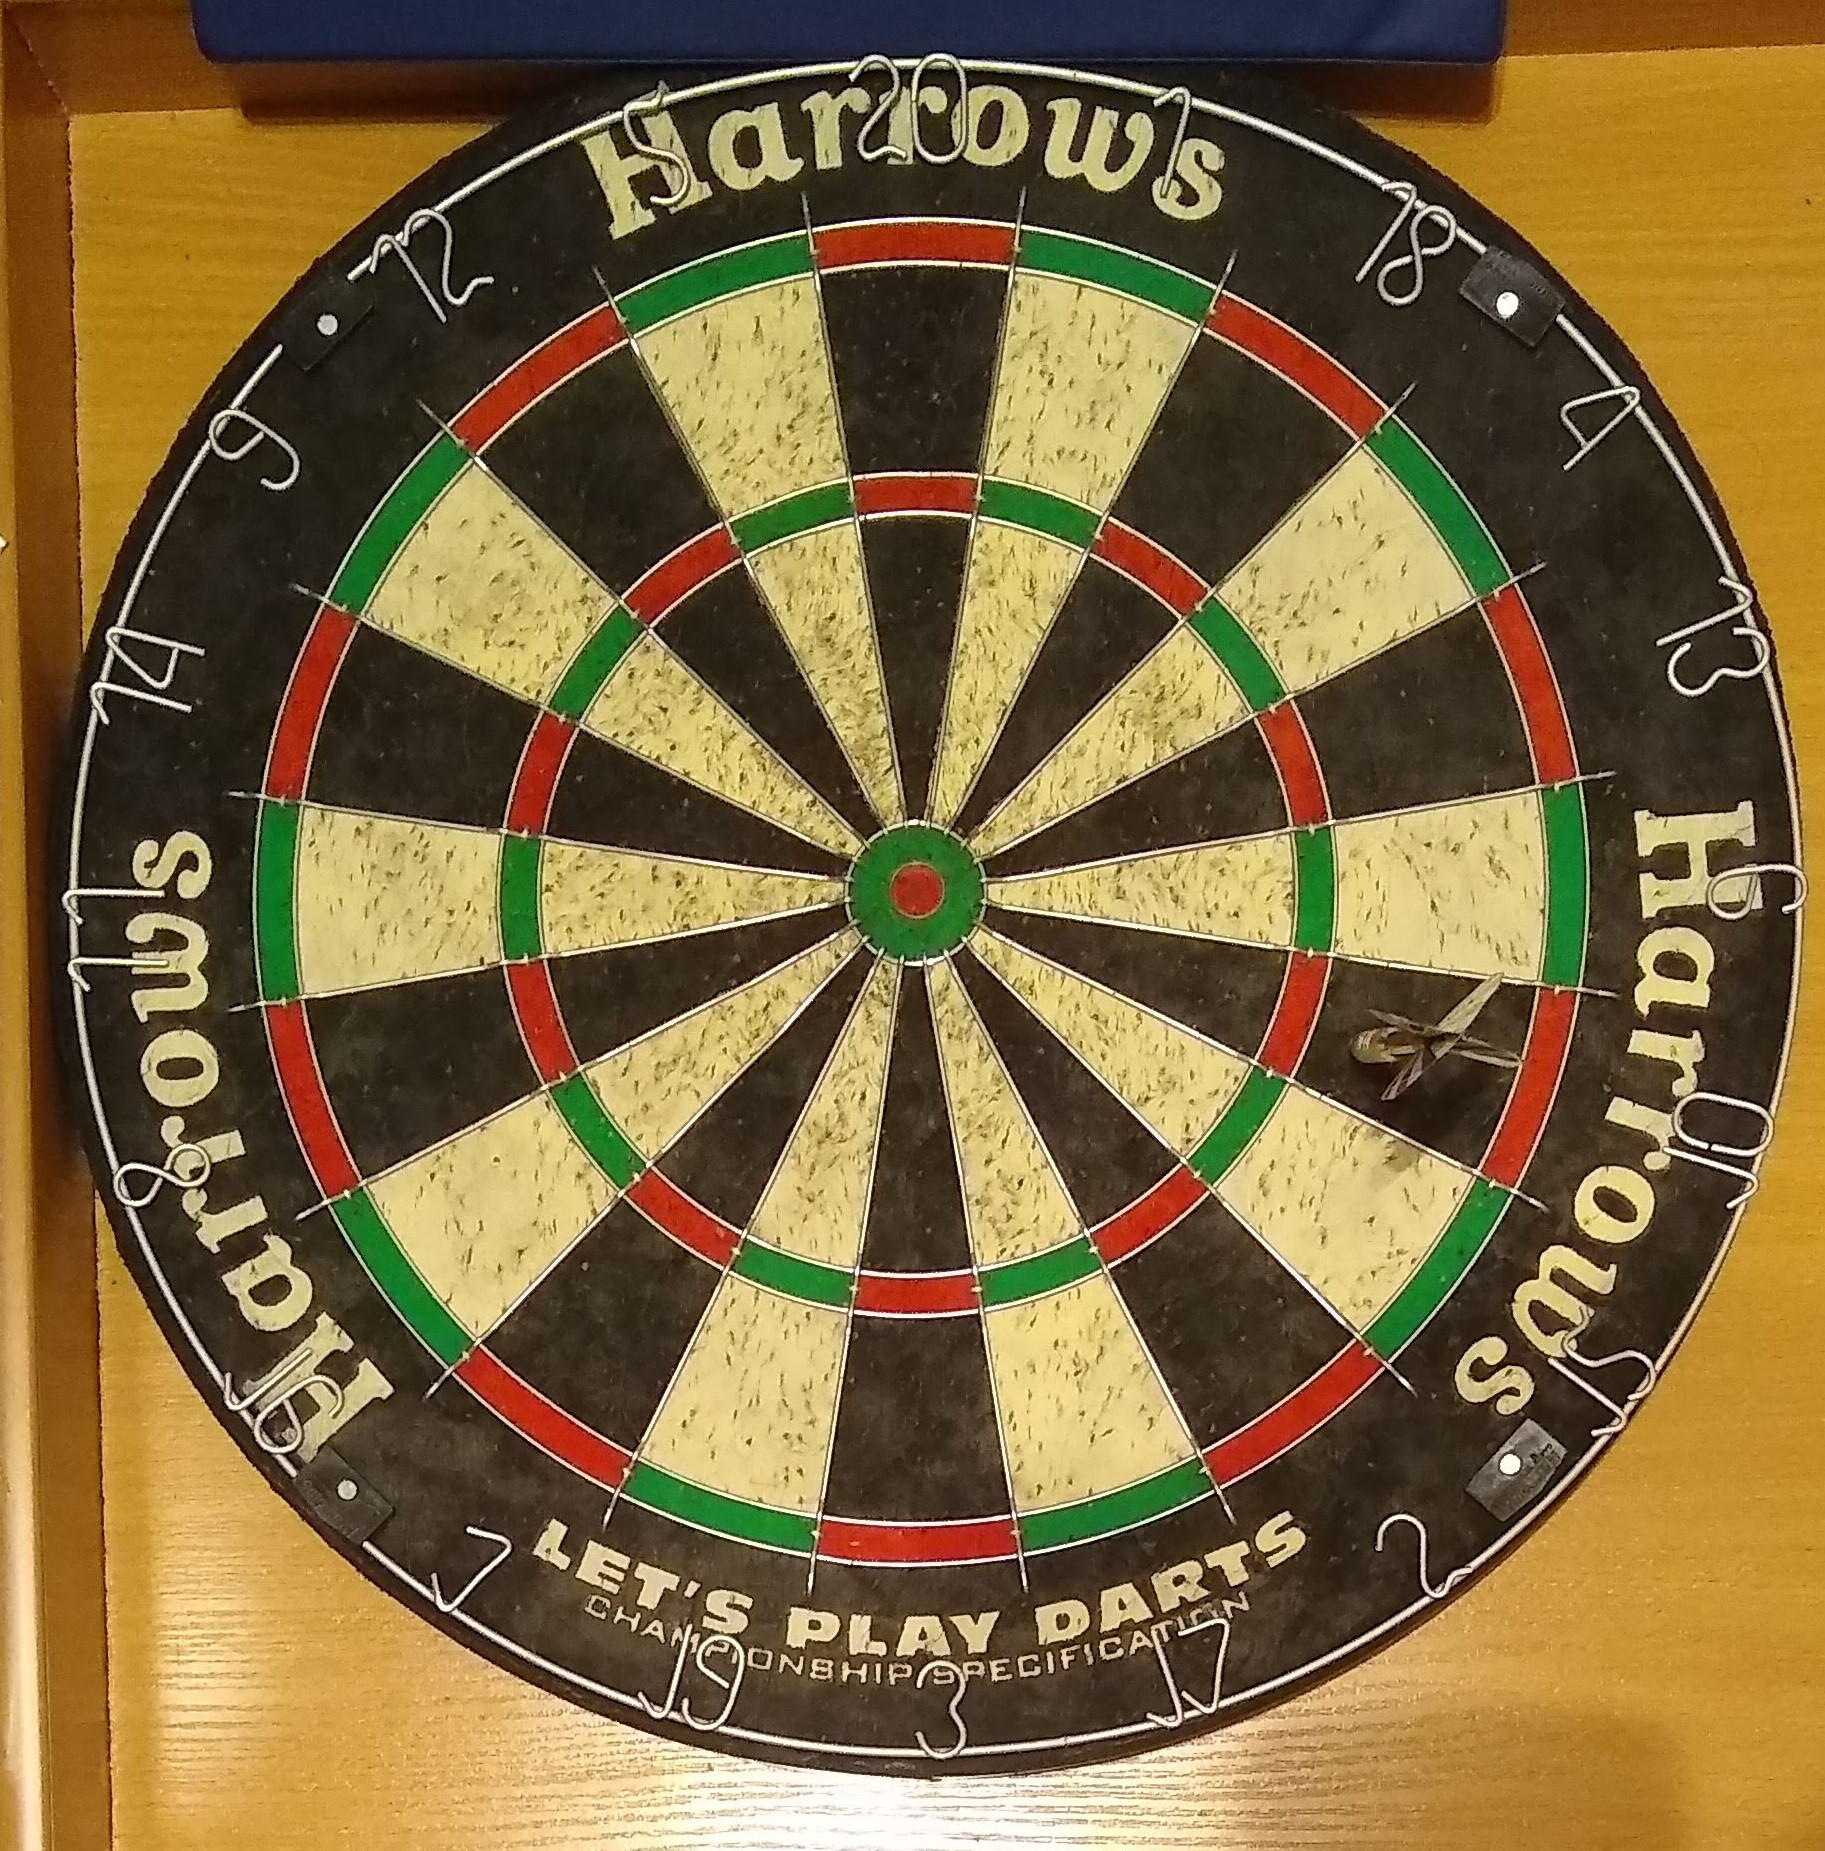
\includegraphics[width=0.5\textwidth]{obrazki/rzutka_gora.jpg}
\end{center}
\captionsource{{\color{dgray}Rzutka wbita w tarczę (rzut z góry)}}{Opracowanie własne}
\label{rzutka_gora}
\end{figure} 

\begin{figure}[h!]
\centering
\begin{subfigure}{\textwidth}
  \centering
  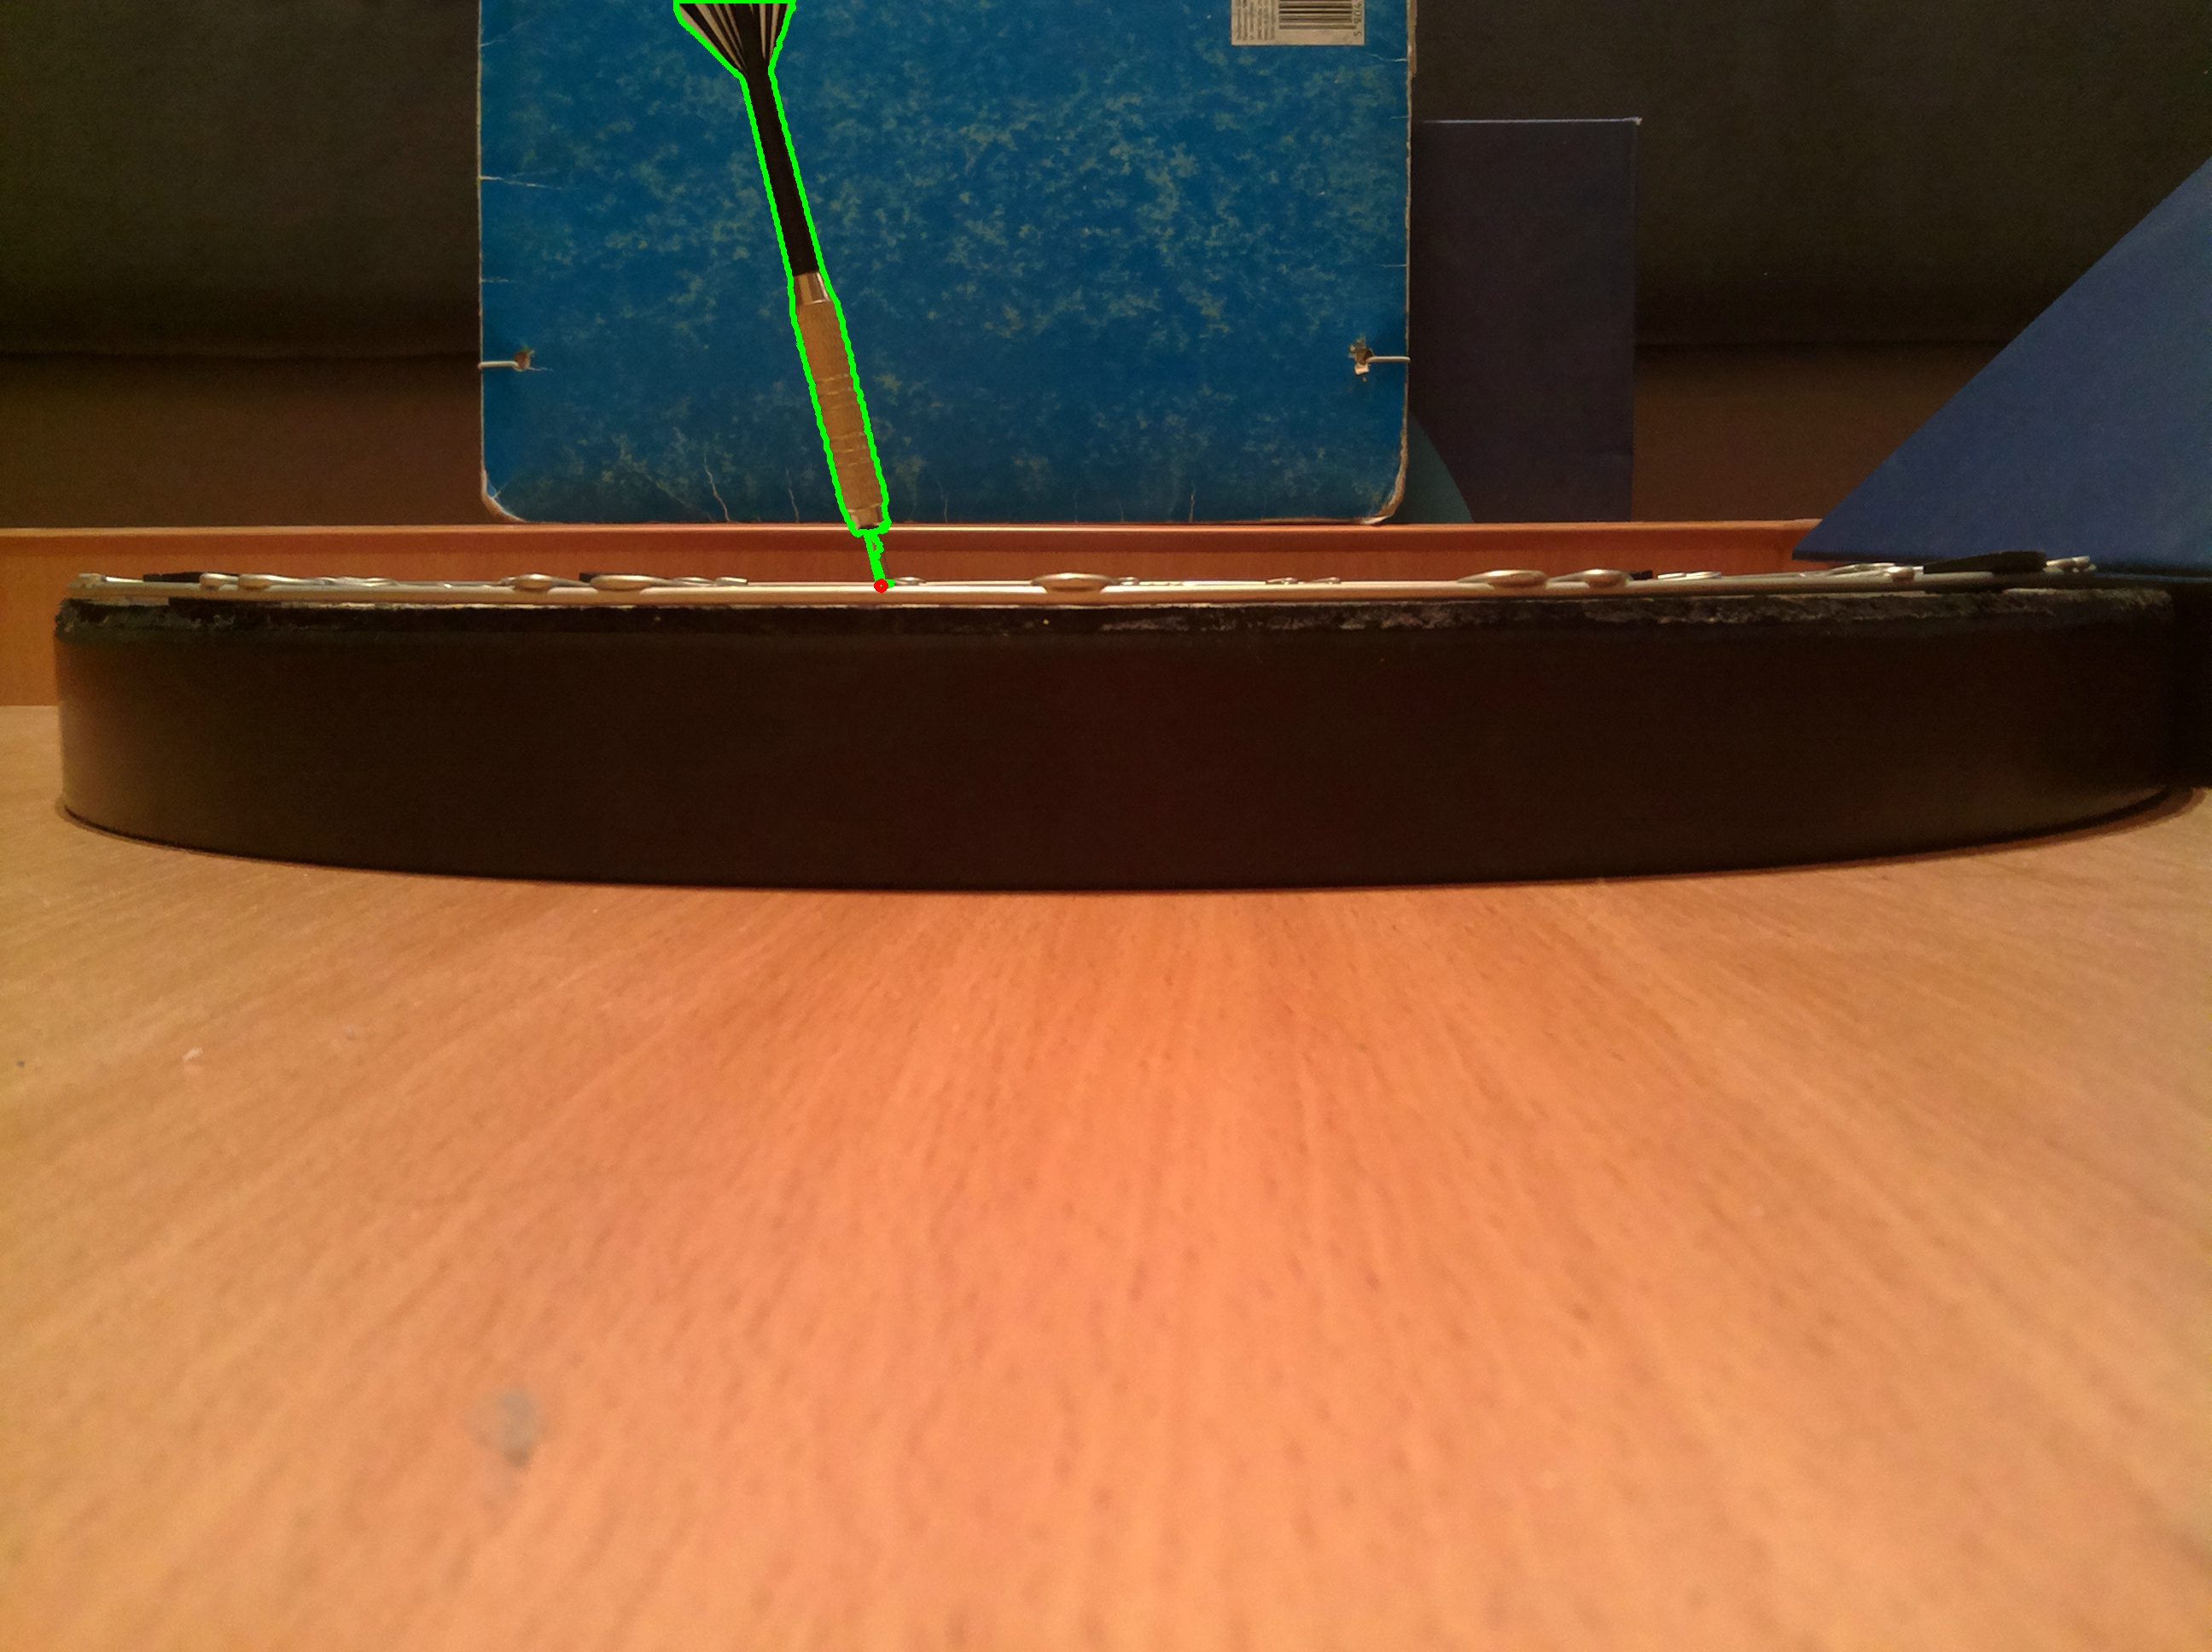
\includegraphics[width=0.75\textwidth]{obrazki/rzutka_pi0.jpg}
  \captionsource{{\color{dgray}Widok z prawej kamery}}{Opracowanie własne}
  \label{rzutka_pi0}
\end{subfigure}
\begin{subfigure}{\textwidth}
  \vspace{0.5cm}
  \centering
  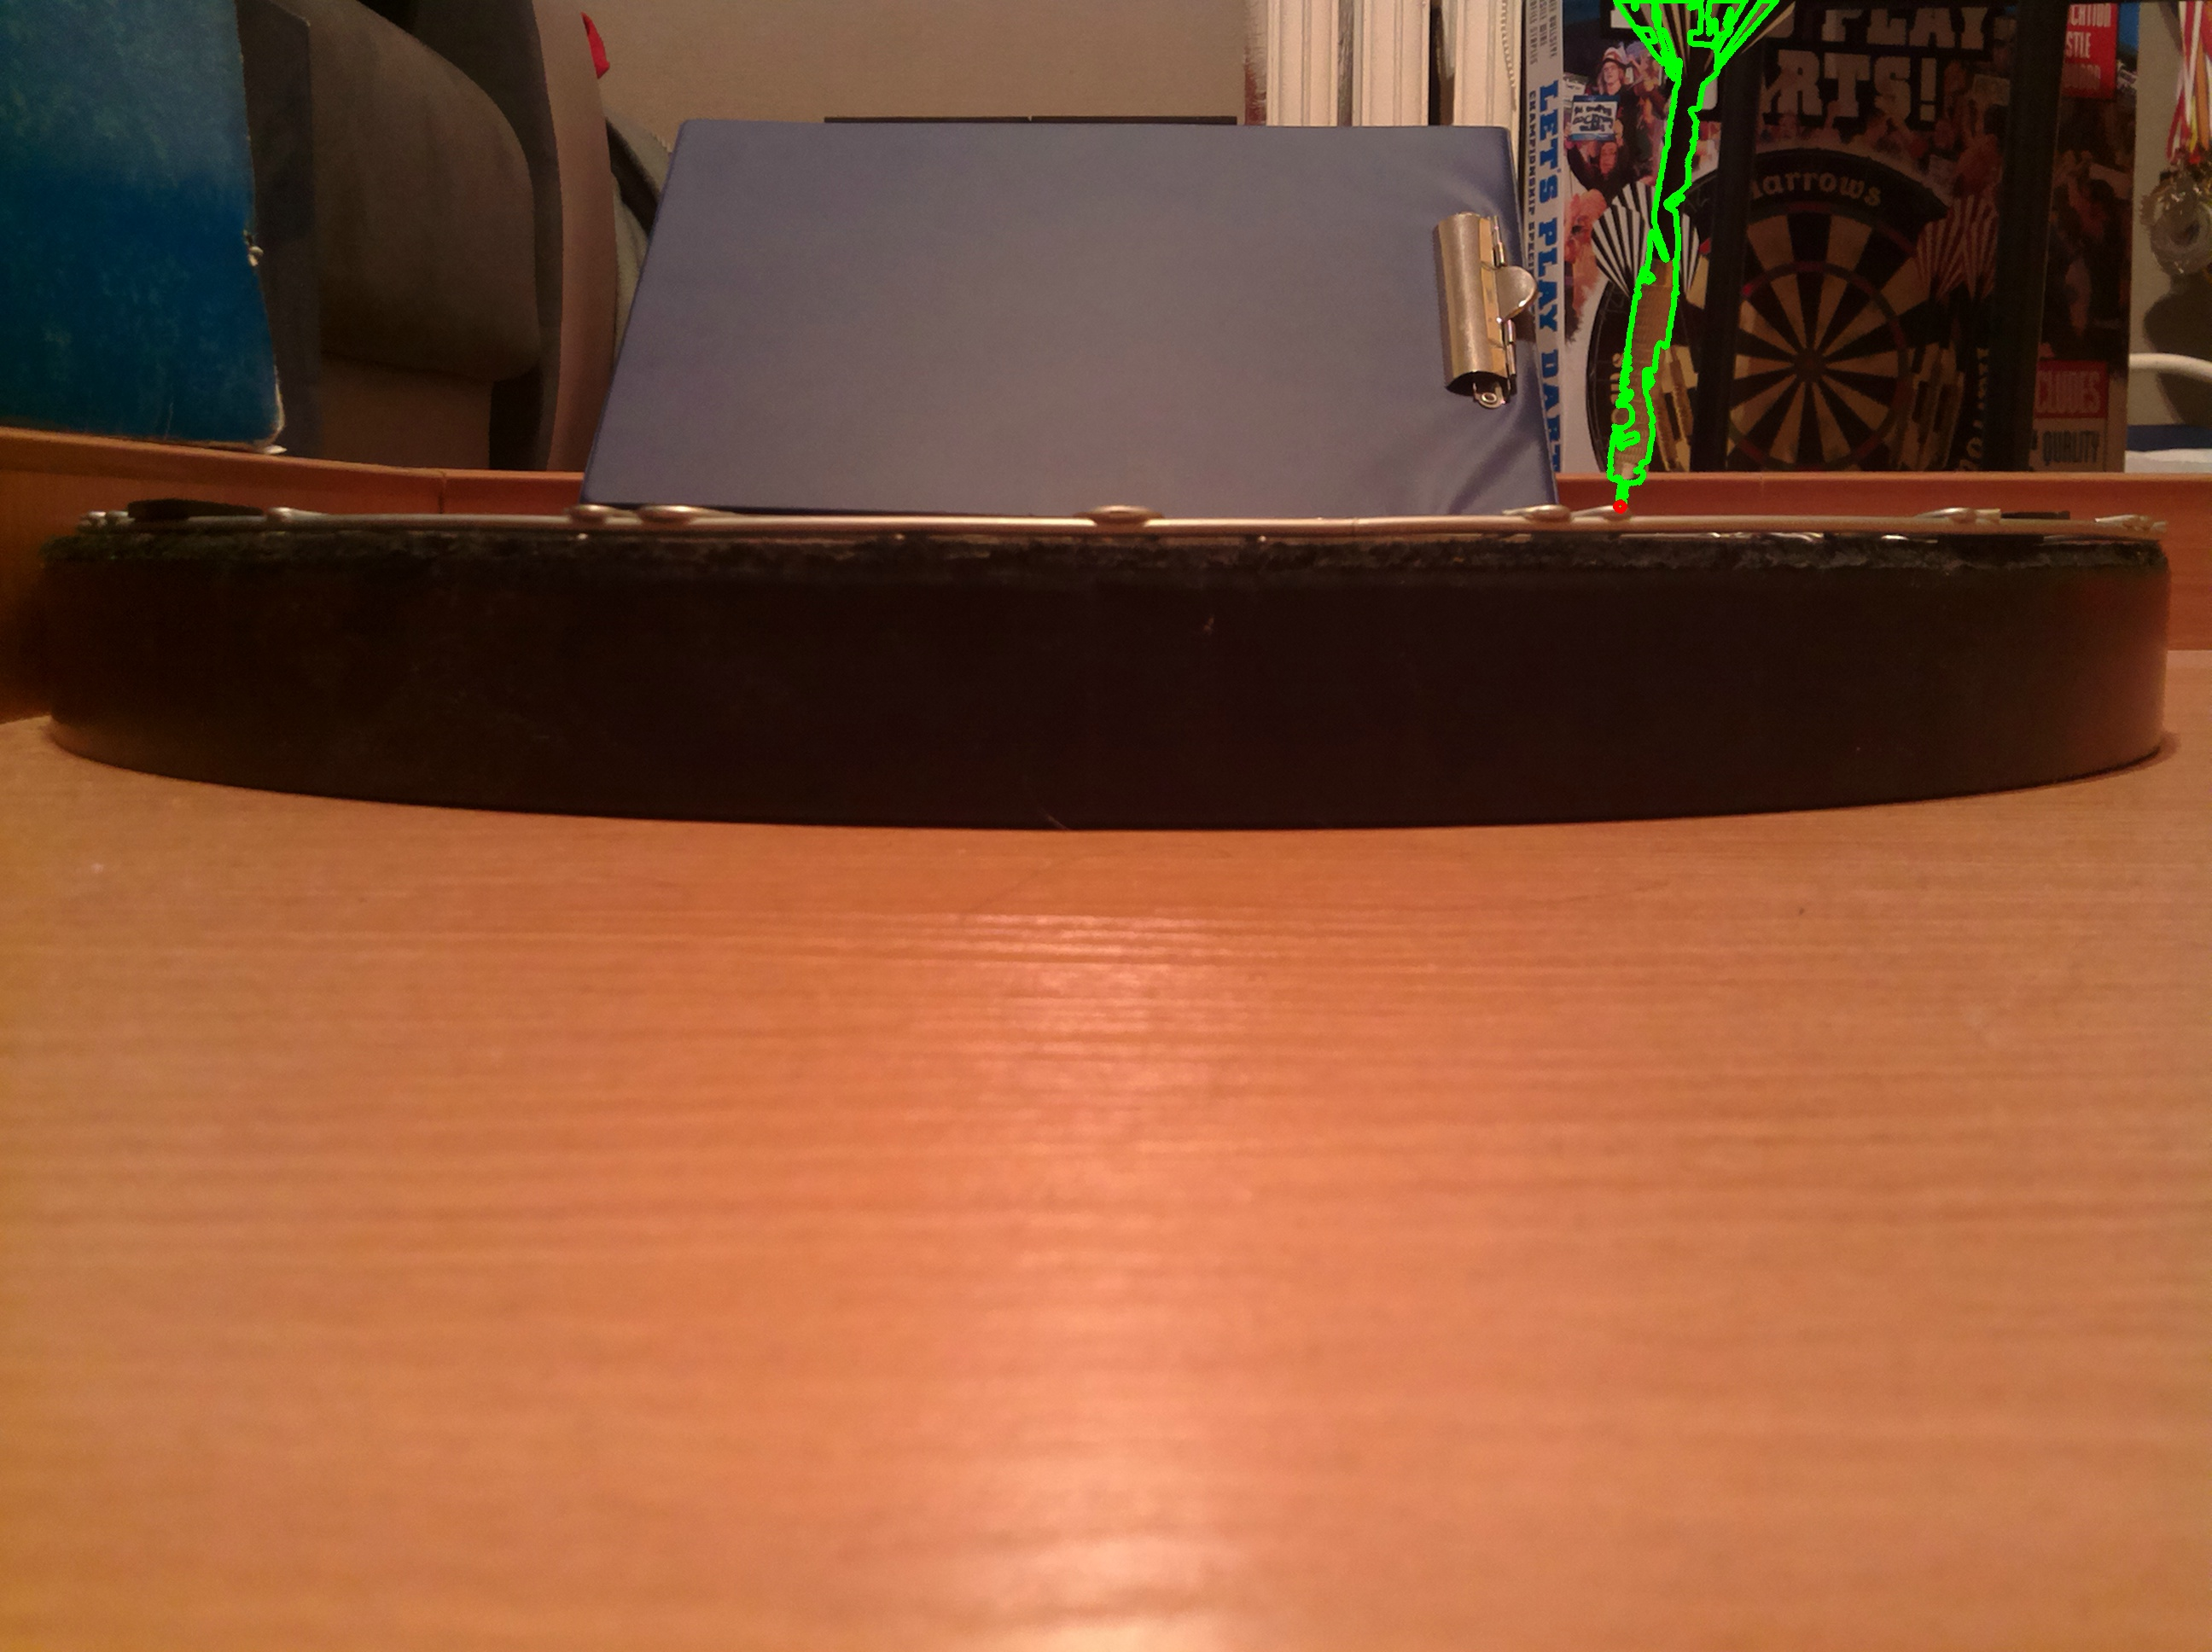
\includegraphics[width=0.75\textwidth]{obrazki/rzutka_pi4.jpg}
  \captionsource{{\color{dgray}Widok z dolnej kamery}}{Opracowanie własne}
  \label{rzutka_pi4}
\end{subfigure}
\caption{Wykrycie konturu rzutki}
\label{rzutka_kontury}
\end{figure}

\begin{figure}[h!]
\begin{center}
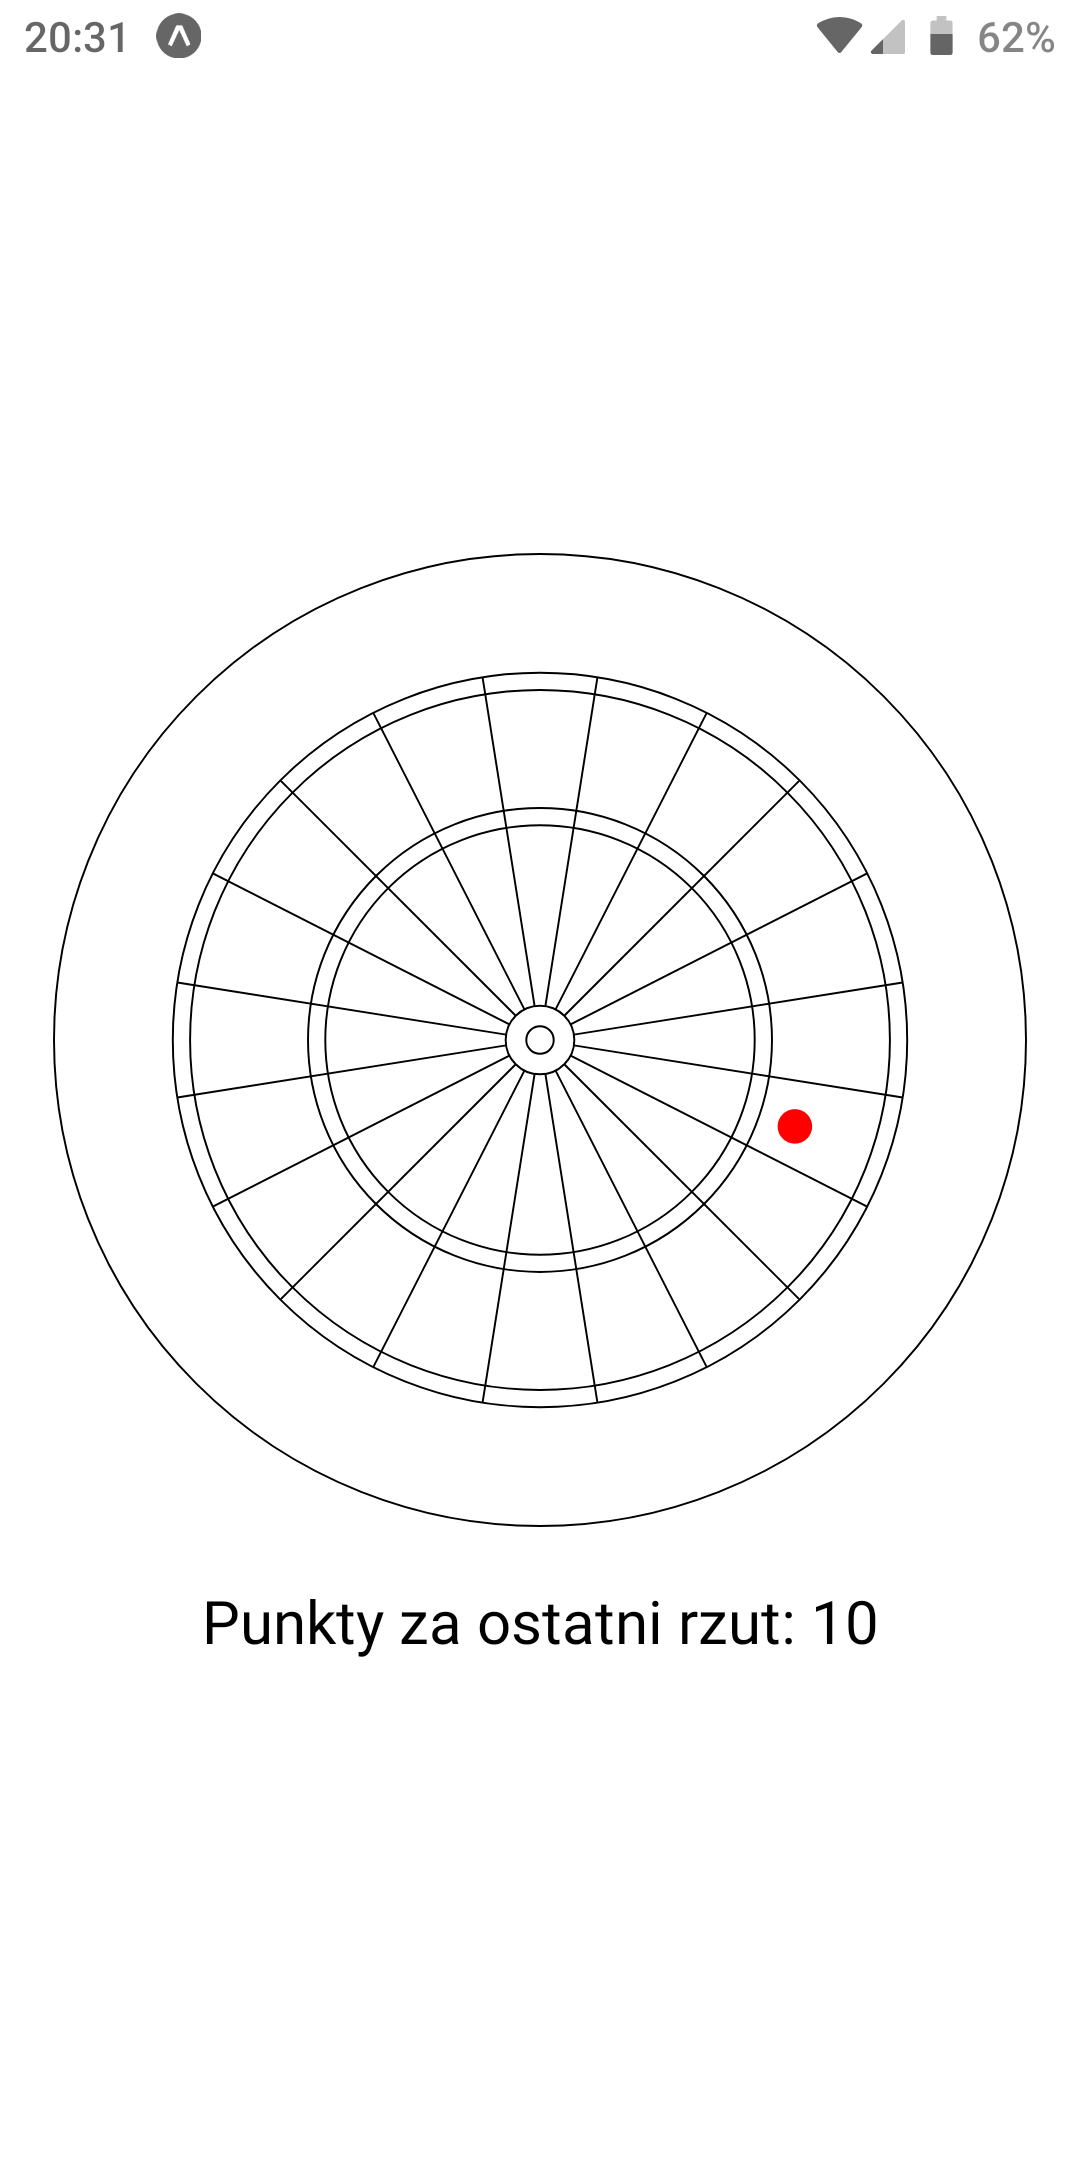
\includegraphics[width=0.3\textwidth]{obrazki/screenshot.png}
\end{center}
\captionsource{{\color{dgray}Zrzut ekranu z aplikacji mobilnej}}{Opracowanie własne}
\label{screenshot}
\end{figure} 

\section{Testy}
TODO
\section{Problemy}
Podczas tworzenia systemu natrafiono na szereg problemów, m.in:
\begin{itemize}
  \item ograniczone zasoby \verb|Raspberry Pi Zero|, powodujące przerywanie programu przy dużym obciążeniu.
  \item mało skuteczne wykrywanie rzutki, gdy tło miało podobny kolor do koloru lotki. Z tego powodu za stelażem ustawiono prowizoryczne zasłony o odmiennych kolorach. Przez długi czas skuteczność obniżała również zbyt wczesna (tj. wykonana przed odjęciem tła) konwersja obrazu do skali szarości, powodująca stratę informacji.
  \item instalacja biblioteki OpenCV, która (w przypadku kompilacji bezpośrednio ze źródeł), trwała na \verb|Pi Zero| ok. 20 godzin.
  \item ustawienie rozdzielczości zdjęcia -- okazało się, że szerokość i wysokość muszą być wielokrotnościami 16.
  \item słaba jakość zdjęć -- przed użyciem i poprawną konfiguracją picamera, zdjęcia wykonywane w trakcie działania systemu były wyraźnie gorszej jakości niż te, wykonane statycznie, np. programem \verb|raspistill|.
\end{itemize}
\section{Prowadzenie projektu}
Projekt był tworzony z użyciem systemu kontroli wersji Git, a zdalne repozytorium znajduje się na portalu GitHub \footnote{Adres: \url{www.github.com}}. Umożliwiło to wygodną, jednoczesną pracę nad różnymi elementami programu, a także zapewniało bezpieczeństwo w przypadku ewentualnych pomyłek.

W celu udokumentowania procesu analizy i tworzenia systemu, a także wykonania implementacji na czas, wykorzystano funkcjonalności portalu GitHub do tworzenia tablic projektowych (ang. \textit{Kanban board}), do których systematycznie były dołączane nowe zadania. Wyznaczano również kamienie milowe, które wskazywały, w jakim miejscu znajduje się projekt. 
	\cleardoublepage
	
	\chapter{Instalacja i wdrożenie}
\label{installation}
\thispagestyle{chapterBeginStyle}

System jest dość specyficzny, dlatego trudno o łatwy sposób wdrożenia go ponownie, głównie z powodu konieczności wykonania stelaża, skonfigurowania urządzeń i zamontowania kamer. Mimo tego, starano się maksymalnie uprościć i zautomatyzować proces tworzenia i uruchamiania systemu.

Do uruchomienia programu na \verb|Pi 4| oraz \verb|Pi Zero| wymagane jest zainstalowanie interpretera języka Python w wersji 3.7 lub wyższej oraz programu \verb|pip3|. Lista pozostałych zależności zapisana w pliku \\ \verb|requirements.txt|, którego można użyć do wygodnej instalacji:
\newline \newline
\indent \verb|cd pi-darts/rpi| \newline
\indent \verb|pip3 install -r requirements.txt|
\newline \newline
\noindent Następnie, by uruchomić program, należy posłużyć się komendami: \newline \newline
\indent \verb|cd src| \newline
\indent \verb|python3 main_pi4.py| (dla \verb|Pi 4|) \newline\newline oraz \indent \newline \newline \indent \verb|cd src| \newline \indent \verb|python3 main_pi0.py| (dla \verb|Pi Zero|) \newline

Warto wspomnieć w tym miejscu o skrypcie \verb|sync.sh|, który został napisany w celu łatwiejszej pracy nad rozwijaniem kodu źródłowego. Dzięki niemu można tworzyć oprogramowanie na komputerze np. z systemem Windows, a wszystkie pliki automatycznie, po każdym zapisie, przeniosą się na urządzenie Raspberry za pomocą protokołu SCP. Wywołanie wygląda następująco:
\newline \newline
\indent \verb|./sync.sh <adres_IP_urządzenia> [<ścieżka do klucza RSA>]|
\newline

Do uruchomienia aplikacji mobilnej wymagane jest posiadanie środowiska Node.js w wersji 12 lub wyższej. 

\noindent Instalacja potrzebnych zależności:
\newline \newline
\indent \verb|cd pi-darts/app| \newline
\indent \verb|npm install -g expo-cli| \newline
\indent \verb|npm install| \newline

\noindent Uruchomienie aplikacji mobilnej:
\newline \newline
\indent \verb|npm start| 

	\cleardoublepage
	
	\chapter{Podsumowanie}
\thispagestyle{chapterBeginStyle}

Udało się sprostać prawie wszystkim wymaganiom funkcjonalnym systemu. Zakończono prace implementacyjne nad pierwszą wersją zarówno aplikacji mobilnej, jak i części serwerowej. System zapewnia skuteczność na wysokim poziomie, choć nadal możliwym do poprawy, tak by jego użycie w trakcie treningu lub zawodów darta było rzeczywistym ułatwieniem procesu obliczania punktów. Pozostaje dużo funkcjonalności i usprawnień, których wykonanie w przyszłości zwiększy użyteczność aplikacji:
\begin{itemize}
  \item umożliwienie przeprowadzenia pełnej rozgrywki (np. w grę \textit{501}) z pomocą systemu, a nie jedynie przekazywania informacji o pojedynczym rzucie;
  \item rozwój metody znajdowania rzutki na zdjęciu, tak by program był mniej wrażliwy np. na zmianę oświetlenia;
  \item zbadanie, na ile kalibracja kamery może poprawić dokładność;
  \item przeprowadzenie większej liczby testów w celu ustalenia optymalnych wartości parametrów oraz wykrycia głównych problemów;
  \item napisanie testów jednostkowych.
  
\end{itemize}

Największym sukcesem pracy jest udane połączenie działań z wielu dziedzin, zarówno matematycznych, jak i czysto informatycznych. Z tego również powodu, w procesie od analizy problemu, przez wykonanie stelaża, aż do implementacji, należało wykazać się dużym przekrojem umiejętności. Znaczącą wartością pracy są również autorskie obliczenia, które okazały się dość skomplikowane, mimo iż oparte są na fundamentalnych prawach geometrii. 
	\cleardoublepage
	
	
	%%%%%%%%%%%%%%%%%%%%%%%%%%%%%%%%%%%%%%%%%%%%%%%%%%%%%%%%%%%%%%%%%%%%%%%%%%%%%%
	%%%%%%%%%%%%%%%%%%%%%%%%%%%%%%% BIBLIOGRAFIA %%%%%%%%%%%%%%%%%%%%%%%%%%%%%%%%%
	%%%%%%%%%%%%%%%%%%%%%%%%%%%%%%%%%%%%%%%%%%%%%%%%%%%%%%%%%%%%%%%%%%%%%%%%%%%%%%
	\nocite{*} % wypisz wszystkie elementy z pliku .bib, niecytowane również

	\pagestyle{bibliographyStyle}
	\bibliographystyle{plabbrv}
	\bibliography{literatura}
	\thispagestyle{chapterBeginStyle}
        \addcontentsline{toc}{chapter}{Bibliografia}

	\cleardoublepage
	
	%%%%%%%%%%%%%%%%%%%%%%%%%%%%%%%%%%%%%%%%%%%%%%%%%%%%%%%%%%%%%%%%%%%%%%%%%%%%%%
	%%%%%%%%%%%%%%%%%%%%%%%%%%%%%%%%% DODATKI %%%%%%%%%%%%%%%%%%%%%%%%%%%%%%%%%%%%
	%%%%%%%%%%%%%%%%%%%%%%%%%%%%%%%%%%%%%%%%%%%%%%%%%%%%%%%%%%%%%%%%%%%%%%%%%%%%%%
	
	\appendix
	\pagestyle{appendixStyle}
	
	\chapter{Zawartość płyty CD}
\thispagestyle{chapterBeginStyle}
\label{plytaCD}

Na dołączonej płycie CD znajduje się projekt \verb|pi-darts|, którego struktura została opisana w podrozdziale \ref{structure}, a sposób instalacji w rozdziale \ref{installation}.


	\cleardoublepage

\end{document}

